\documentclass[11pt]{amsart}

%\usepackage[english]{babel}
\usepackage[cp1250]{inputenc}
\usepackage{graphicx}
\usepackage{url}
\usepackage[all]{xy}
\usepackage{multicol}
\usepackage{amsthm}
\usepackage{amsmath}
\usepackage{amssymb}
\usepackage{geometry}
\usepackage{pinlabel}
\usepackage{hyperref}
\usepackage{array}
\usepackage{xcolor}
\usepackage{mathtools}
\usepackage{tikz}
\usetikzlibrary{positioning}
\usepackage{pdflscape}
\usepackage{listofitems}
\usepackage{float}


\newtheorem{Theorem}{Theorem}[section]
\newtheorem{lemma}[Theorem]{Lemma}
\newtheorem{proposition}[Theorem]{Proposition}
\newtheorem{corollary}[Theorem]{Corollary}
\newtheorem*{definition}{Definition}
\newtheorem{remark}[Theorem]{Remark}
\newtheorem{example}[Theorem]{Example}
\newtheorem{notation}[Theorem]{Notation}


\newcommand{\ZZ}{\mathbb {Z}}
\newcommand{\RR}{\mathbb {R}}
\newcommand{\CC}{\mathbb {C}}
\newcommand{\YY}{\mathbb {Y}}
\newcommand{\NN}{\mathbb {N}}
\newcommand{\av}{\mathbf{a}}
\newcommand{\bv}{\mathbf{b}}
\newcommand{\cv}{\mathbf{c}}
\newcommand{\rr}{\mathbf{r}}
\newcommand\cycle[2][\,]{%
  \readlist\thecycle{#2}%
  (\foreachitem\i\in\thecycle{\ifnum\icnt=1\else#1\fi\i})%
}

\setlength{\unitlength}{1cm}



\subjclass[2020]{57K10, 57K18}
\keywords{polygonal link, cube of resolutions, smoothing, Khovanov homology, symmetry, permutation of a smoothing}


\begin{document}


\title{On discrete symmetries of the cube of smoothings}


\author{Eva Horvat}
\address{University of Ljubljana, Faculty of Education, Kardeljeva plo\v s\v cad 16, 1000 Ljubljana, Slovenia, eva.horvat@pef.uni-lj.si}
\email{\href{mailto:eva.horvat@pef.uni-lj.si}{eva.horvat@pef.uni-lj.si}}

\maketitle

\begin{abstract} We study the Khovanov complex of closed piecewise linear curves in $\RR ^3$. A polygonal link representation endows the cube of resolutions with an additional combinatorial structure. The set of symmetries preserving this structure and its quotient under link equivalence are studied. Our results offer new combinatorial ways of computing Khovanov homology and might lead to other group-theoretic invariants of links.
\end{abstract}


\section{Polygonal links}

We are interested in the representation of knots as closed polygonal curves in the Euclidean space. Knots admitting such representation are called tame, and most techniques of knot theory apply to tame knots. Here we recall some basic notions that may also be found in \cite{LIV}.

\begin{definition} For an integer $n\geq 3$, let $(p_{1},p_{2},\ldots ,p_{n})$ be an $n$-tuple of distinct points $p_{i}\in \RR ^{3}$ for $i=1,2,\ldots ,n$, such that:\begin{enumerate}
\item no three subsequent points $p_{i-1},p_{i},p_{i+1}$ are collinear,
\item any two distinct edges $\overline{p_{i}p_{i+1}}$ and $\overline{p_{j}p_{j+1}}$ may only intersect at a common endpoint.
\end{enumerate} Here the vertex indices are computed modulo $n$ in the sense that $p_{n+1}=p_{1}$. The union $\bigcup _{i=1}^{n}\overline{p_{i}p_{i+1}}$ will be called the \textbf{polygonal knot} $(p_{1},p_{2},\ldots ,p_{n})$. Points $p_{i}$ are called the \textbf{vertices} and segments $\overline{p_{i}p_{i+1}}$ are called the \textbf{edges} of the polygonal knot. 
\end{definition}

Observe that the order of vertices induces a natural orientation of a polygonal knot. Moreover, the cyclic permutation $\sigma =(1\,2\,3\ldots n)\in S_n$ of the vertex indices leaves the polygonal knot invariant, that is, the $n$-tuples $(p_{1},p_{2},\ldots ,p_{n})$ and $(p_{\sigma ^{k}(1)},p_{\sigma ^{k}(2)},\ldots ,p_{\sigma ^{k}(n)})$ define the same polygonal knot for any $k\in \{0,1,\ldots ,n-1\}$. 

\begin{definition} A polygonal knot $J$ is called a \textbf{deformation} of a polygonal knot $K$ if any one of these two knots is given by the tuple $(p_{1},p_{2},\ldots ,p_{n})$ and the other one is given by the tuple $(p_{1},p_{2},\ldots ,p_{n+1})$, where the triangle with vertices $p_{1}$, $p_{n}$, $p_{n+1}$ intersects the knot $(p_{1},p_{2},\ldots ,p_{n})$ exactly in the line segment $\overline{p_{1}p_{n}}$. 

Two knots $K$ and $L$ are called \textbf{equivalent} if there exists a sequence of knots $K=K_0$, $K_1$, \ldots , $K_{n}=L$, where $K_{i+1}$ is a deformation of the knot $K_i$ for $i=0,1, \ldots ,n-1$. 
\end{definition}

A polygonal knot in the above definition has an obvious piecewise linear parametrization $\rr \colon [0,n]\to \RR ^{3}$, given by $$\rr (t)=\left (t-\lfloor t\rfloor \right )p_{\lceil t\rceil}+\left (1-t+\lfloor t\rfloor \right )p_{\lceil t\rceil +1}\;.$$

A union of pairwisely disjoint polygonal knots is called a \textbf{polygonal link}. Given nonnegative integers $0=n_{0}<n_{1}<n_{2}<\ldots <n_{r}=n$, a polygonal link may be given as a sequence $$\left ((p_{n_0+1},\ldots ,p_{n_{1}}),(p_{n_{1}+1},\ldots ,p_{n_{2}}),\ldots (p_{n_{r-1}+1},\ldots ,p_{n_r})\right )$$ of tuples of points in the Euclidean space, each tuple defining one link component. Observe that any cyclic permutation $\sigma _{i}=\cycle{n_{i-1}+1,n_{i-1}+2,\ldots ,n_{i}}\in S_n$ of the vertex indices leaves the polygonal link invariant for  $i\in \{1,\ldots ,r\}$. Once we have fixed the sequence of points $(p_{1},p_{2},\ldots ,p_{n})$, the link is completely determined by the permutation $\sigma =\sigma _{1}\sigma _{2}\ldots \sigma _{r}$ which maps the index of any vertex to the index of the next vertex in its component of the polygonal link.  

\begin{definition} Let the sequence $$\left ((p_{n_0+1},\ldots ,p_{n_{1}}),(p_{n_{1}+1},\ldots ,p_{n_{2}}),\ldots (p_{n_{r-1}+1},\ldots ,p_{n_r})\right )$$ of tuples of points in $\RR ^{3}$ define a polygonal link $L=\bigcup _{i=0}^{r-1}\left (\left (\bigcup _{j=n_{i}+1}^{n_{i+1}}\overline{p_{j}p_{j+1}}\right )\cup \overline{p_{n_{i+1}}p_{n_{i}+1}}\right )$. A projection $\pi \colon L\to \Sigma $ of the link $L$ to an affine plane $\Sigma \subset \RR ^3$ is called \textbf{regular} if \begin{enumerate}
\item no three points of $L$ map to the same image,  
\item there are finitely many isolated double points,
\item no vertex of $L$ maps to a double point of $\pi $. 
\end{enumerate} The image of a regular projection, endowed with the ''crossing information`` at every double point, is called a \textbf{link diagram} of the polygonal link $L$. The double points in a link diagram are called \textbf{crossings}. A link diagram is called \textbf{good} if the image of every edge contains at most one crossing. 
\end{definition}

Figure \ref{fig1} shows a good diagram of a polygonal trefoil knot with nine vertices.

\begin{figure}[H]
\begin{center}
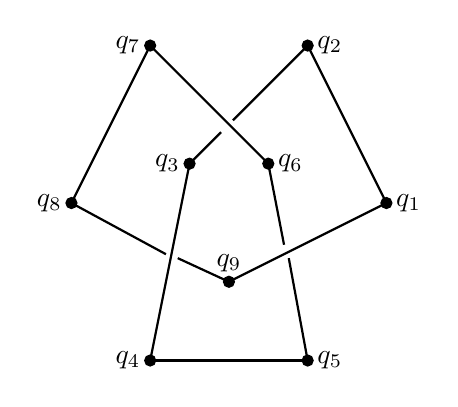
\begin{tikzpicture}
\draw[black, thick](-1,2) -- (-2,0);
\draw[black, thick](-2,0) -- (-0.8,-0.65);
\draw[black, thick](-0.65,-0.7) -- (0,-1);
\draw[black, thick](0,-1) -- (2,0);
\draw[black, thick](2,0) -- (1,2);
\draw[black, thick](1,2) -- (0.05,1.05);
\draw[black, thick](-0.1,0.9) -- (-0.5,0.5);
\draw[black, thick](-0.5,0.5) -- (-1,-2);
\draw[black, thick](-1,-2) -- (1,-2);
\draw[black, thick](0.5,0.5) -- (-1,2);
\draw[black, thick](0.5,0.5) -- (0.7,-0.53);
\draw[black, thick](0.76,-0.7) -- (1,-2);
\filldraw[black] (-1,2) circle (2pt) node[anchor=east]{$q_{7}$};
\filldraw[black] (-2,0) circle (2pt) node[anchor=east]{$q_{8}$};
\filldraw[black] (0,-1) circle (2pt) node[anchor=south]{$q_{9}$};
\filldraw[black] (2,0) circle (2pt) node[anchor=west]{$q_{1}$};
\filldraw[black] (1,2) circle (2pt) node[anchor=west]{$q_{2}$};
\filldraw[black] (-0.5,0.5) circle (2pt) node[anchor=east]{$q_{3}$};
\filldraw[black] (-1,-2) circle (2pt) node[anchor=east]{$q_{4}$};
\filldraw[black] (1,-2) circle (2pt) node[anchor=west]{$q_{5}$};
\filldraw[black] (0.5,0.5) circle (2pt) node[anchor=west]{$q_{6}$};
\end{tikzpicture}
\end{center}
\caption{A good diagram of a trefoil knot}
\label{fig1}
\end{figure}

\begin{lemma} Every polygonal link is equivalent to a polygonal link admitting a good link diagram. 
\end{lemma}
\begin{proof} Suppose a polygonal link $L$ is given by a sequence $$\left ((p_{1},\ldots ,p_{n_{1}}),(p_{n_{1}+1},\ldots ,p_{n_{2}}),\ldots (p_{n_{r-1}+1},\ldots ,p_{n_r})\right )$$ of tuples of points in $\RR ^{3}$ and denote $n=n_r$. Let $\pi \colon L\to \Sigma $ be the projection of $L$ onto a plane $\Sigma $ in the direction of a vector $\mathbf{v}\in \RR ^{3}$. Observe that:\begin{enumerate}
\item if $\pi (p_i)=\pi (p_j)$ for $i\neq j\in \{1,2,\ldots ,n\}$, then $\mathbf{v}\in Lin\{p_{i},p_{j}\}$.  
\item if $\pi (p_{j})=\pi ((1-t)p_{i}+tp_{i+1})$ for $i\neq j\in \{1,2,\ldots ,n\}$, then $\mathbf{v}\in Lin\{p_{i},p_{i+1},p_{j}\}$. 
\item if $\pi ((1-t_{i})p_{i}+t_{i}p_{i+1})=\pi ((1-t_{j})p_{j}+t_{j}p_{j+1})=\pi ((1-t_{k})p_{k}+t_{k}p_{k+1})$, then $\mathbf{v}\in Lin\{p_{i},p_{i+1},(1-t_{j})p_{j}+t_{j}p_{j+1}\}\cap Lin\{p_{k},p_{k+1},(1-t_{j})p_{j}+t_{j}p_{j+1}\}$.  
\end{enumerate}
For $i\neq j\in \{1,2,\ldots ,n\}$, denote by $\Sigma _{i,j}=Lin\{p_{i},p_{i+1},p_{j}\}$ the affine plane in $\RR ^3$, containing the vertices $p_{i},p_{i+1}$ and $p_{j}$. For three pairwise distinct indices $i,j,k\in \{1,2,\ldots ,n\}$, let $(t_{i},t_{j},t_{k})\in [0,1]^{3}$ denote the solution to the linear system 
\begin{xalignat*}{1}
& \left ((1-t_{i})p_{i}+t_{i}p_{i+1})-((1-t_{j})p_{j}+t_{j}p_{j+1})\right )\times \left ((1-t_{i})p_{i}+t_{i}p_{i+1})-((1-t_{k})p_{k}+t_{k}p_{k+1})\right )=0
\end{xalignat*} if it exists, and let $(t_{i},t_{j},t_{k})=(-1,-1,-1)$ otherwise. Let $A=\bigcup _{i\neq j\in \{1,2,\ldots ,n\}}\Sigma _{i,j}$ and 
\begin{xalignat*}{1}
& B=\{Lin\{(1-t_{i})p_{i}+t_{i}p_{i+1})-((1-t_{j})p_{j}+t_{j}p_{j+1})\}\,|\\
& \, i\neq j\in \{1,2,\ldots n\} \textrm{ and $(t_{i},t_{j},t_{k})\neq (-1,-1,-1)$ for some }k\in \{1,2,\ldots ,n\}\backslash \{i,j\} \}\;.\end{xalignat*}
If $\mathbf{v}\notin B$, then the projection $\pi $ has no triple points. If $\mathbf{v}\notin A\cup B$, then $\pi $ is a regular projection. The set $A\cup B$ is a union of a finite number of affine planes and lines in $\RR ^3$ and its complement $\RR ^{3}\backslash (A\cup B)$ is a nonempty open subset (a submanifold of codimension 0). Therefore, we may choose a vector $\mathbf{v}$ so that $\pi $ is a regular projection. 

Let $\pi \colon L\to \Sigma $ be a regular projection in the direction of a vector $\mathbf{v}$, defining a link diagram $\pi (L)$. Denote by $e_{i}=\overline{p_{i}p_{i+1}}$ the $i$-th edge of $L$ and suppose that the image $\pi (e_i)$ contains two crossings at points $\pi (c_{j})=\pi ((1-t_{j})p_{i}+t_{j}p_{i+1})$ for $j=1,2$. Let $\epsilon =\min \left \{|\frac{c_{1}+c_{2}}{2}-x|\,\colon \, x\in L\backslash Int(e_{i})\right \}$ and denote $y=\frac{(p_{i+1}-p_{i})\times \mathbf{v}}{|(p_{i+1}-p_{i})\times \mathbf{v}|}$. Apply a deformation of $L$ by adding a new vertex $\left (\frac{c_{1}+c_{2}}{2}+\frac{\epsilon }{2}y\right )$ between the vertices $p_{i}$ and $p_{i+1}$. Repeating this procedure for every edge of $L$ whose projection contains more than one crossing, we obtain a good diagram of $L$.  
\end{proof}

Suppose we have a good link diagram $\pi \colon L\to \Sigma $ of a polygonal link $$\left ((p_{n_0+1},\ldots ,p_{n_{1}}),(p_{n_{1}+1},\ldots ,p_{n_{2}}),\ldots (p_{n_{r-1}+1},\ldots ,p_{n_r})\right )$$ with $r$ components and $n=n_{r}$ vertices. Choose a suitable isometry $h\colon \Sigma \to \RR ^2$ from the projection plane to the standard Euclidean plane. Then the diagram may be described by the tuple $$\left ((q_{n_0+1},\ldots ,q_{n_{1}}),(q_{n_{1}+1},\ldots ,q_{n_{2}}),\ldots (q_{n_{r-1}+1},\ldots ,q_{n_r})\right )\;,$$ where $q_{i}=h(\pi (p_{i}))$. Denote by $k$ the number of crossings of this diagram. Since each edge contains at most one crossing and each crossing is contained in two edges, we have $n\geq 2k$. \\

\begin{figure}[H]
\begin{tikzpicture}
\matrix [column sep=1cm]
{
\node {\begin{tikzpicture}
\draw[black, thick][<-] (-1,-1) -- (1,1);
\draw[black, thick] (-1,1) -- (-0.1,0.1);
\draw[black, thick][->] (0.1,-0.1) -- (1,-1);
\filldraw[black] (-1,1) circle (2pt) node[anchor=east]{$q_{v}$};
\filldraw[black] (1,1) circle (2pt) node[anchor=west]{$q_{i}$};
\filldraw[black] (-1,-1) circle (2pt) node[anchor=east]{$q_{j}$};
\filldraw[black] (1,-1) circle (2pt) node[anchor=west]{$q_{w}$};
\end{tikzpicture}}; & \node {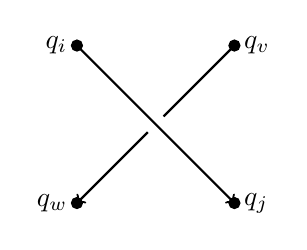
\begin{tikzpicture}
\draw[black, thick][->] (-1,1) -- (1,-1);
\draw[black, thick] (1,1) -- (0.1,0.1);
\draw[black, thick][->] (-0.1,-0.1) -- (-1,-1);
\filldraw[black] (-1,1) circle (2pt) node[anchor=east]{$q_{i}$};
\filldraw[black] (1,1) circle (2pt) node[anchor=west]{$q_{v}$};
\filldraw[black] (-1,-1) circle (2pt) node[anchor=east]{$q_{w}$};
\filldraw[black] (1,-1) circle (2pt) node[anchor=west]{$q_{j}$};
\end{tikzpicture}};\\
};
\end{tikzpicture}
\caption{A positive (left) and a negative crossing (right) of a good diagram}
\label{fig2}
\end{figure}

At each crossing, an overcrossing edge goes over an undercrossing edge. The chosen orientation of the polygonal link induces an orientation of every edge, i.e. the order of its two endpoints. The index of the first (resp. the last) endpoint of an edge will be called ``the starting index'' (resp. ``the ending index''). We first enumerate the crossings: start walking along the diagram starting at $q_{1}$ in the direction induced by the order of the tuple (when we reach the vertex with the highest index of a given component, we need to jump onto the lowest index vertex of the next component). During this walk, we enumerate the crossings in the order we walk along their overcrossing edges (each time we walk along an overcrossing edge, we enumerate its respective crossing by the smallest integer that has not already been taken).

Let us denote by $i_{m}$ (resp. $j_m$)  the starting index (resp. the ending index) of the overcrossing edge of the $m$-th crossing. Thus $1\leq i_{1}\leq i_{2}\leq \ldots \leq i_{k}\leq n$. Let  $v_{m}$ (resp. $w_m$) denote the starting index (resp. the ending index) of the undercrossing edge at the $m$-th crossing. Thus at the $m$-th crossing, the overcrossing edge $\overline{q_{i_{m}}q_{j_{m}}}$ passes above the undercrossing edge $\overline{q_{v_{m}}q_{w_{m}}}$. The starting indices of the overcrossing (resp. undercrossing) edges give rise to two index subsets $\mathcal{I}=\{i_{1},i_{2}, \ldots ,i_{k}\}$ and $\mathcal{V}=\{v_{1},v_{2},\ldots ,v_{k}\}$. Denote $\mathcal{K}=\{1,2,\ldots n\}\backslash (\mathcal{I}\cup \mathcal{V})$. Every vertex of the diagram is either: \begin{itemize}
\item an initial vertex of an overcrossing edge (with index from $\mathcal{I}$),
\item an initial vertex of an undercrossing edge (with index from $\mathcal{V}$),
\item an initial vertex of an edge without crossings (with index from $\mathcal{K}$).
\end{itemize}

The sign of a crossing depends on the chosen orientation of the projection plane. Using the standard normal vector $\mathbf{n}=(0,0,1)$ to the plane $\RR ^{2}\subset \RR ^{3}$, the sign of the $m$-th crossing is given by $$\epsilon _{m}=\frac{((q_{j_{m}}-q_{i_{m}})\times (q_{w_{m}}-q_{v_{m}}))\cdot \mathbf{n}}{\left |((q_{j_{m}}-q_{i_{m}})\times (q_{w_{m}}-q_{v_{m}}))\cdot \mathbf{n}\right |}\;.$$ Figure \ref{fig2} shows the local picture of a positive and a negative crossing. 


\section{Symmetries in the cube of smoothings}

\subsection{Preliminaries on the Khovanov complex}
We review some basics on the construction of the Khovanov complex. A good introduction to Khovanov homology can be found in \cite{BN} or \cite{TUR}.

Suppose we have a good link diagram of a polygonal link. Denote by $k_+$ (resp. $k_{-}$) the number of crossings with a positive (resp. negative) sign and let $k=k_{+}+k_{-}$.  At every crossing, the diagram may be locally transformed (resolved) by a 1-\textbf{smoothing} or a 0-\textbf{smoothing}, see Figure \ref{fig3}.  
\begin{figure}[H]
\begin{tikzpicture}
\matrix
{
\node {\begin{tikzpicture}[scale=0.50]
\draw[black, thick][<-] (-1,-1) -- (1,1);
\draw[black, thick] (-1,1) -- (-0.1,0.1);
\draw[black, thick][->] (0.1,-0.1) -- (1,-1);
\filldraw[black] (-1,1) circle (2pt) node[anchor=east]{$q_{v}$};
\filldraw[black] (1,1) circle (2pt) node[anchor=west]{$q_{i}$};
\filldraw[black] (-1,-1) circle (2pt) node[anchor=east]{$q_{j}$};
\filldraw[black] (1,-1) circle (2pt) node[anchor=west]{$q_{w}$};
\end{tikzpicture}}; & \node{}; & \node {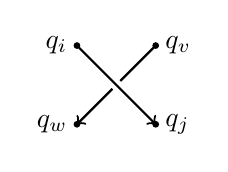
\begin{tikzpicture}[scale=0.50]
\draw[black, thick][->] (-1,1) -- (1,-1);
\draw[black, thick] (1,1) -- (0.1,0.1);
\draw[black, thick] [->](-0.1,-0.1) -- (-1,-1);
\filldraw[black] (-1,1) circle (2pt) node[anchor=east]{$q_{i}$};
\filldraw[black] (1,1) circle (2pt) node[anchor=west]{$q_{v}$};
\filldraw[black] (-1,-1) circle (2pt) node[anchor=east]{$q_{w}$};
\filldraw[black] (1,-1) circle (2pt) node[anchor=west]{$q_{j}$};
\end{tikzpicture}}; \\
\node {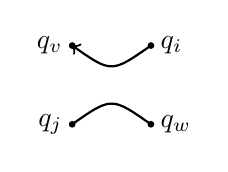
\begin{tikzpicture}[scale=0.50]
\draw[black, thick][<-] (-1,1) .. controls (0,0.3) .. (1,1) ;
\draw[black, thick] (-1,-1) .. controls (0,-0.3) .. (1,-1);
\filldraw[black] (-1,1) circle (2pt) node[anchor=east]{$q_{v}$};
\filldraw[black] (1,1) circle (2pt) node[anchor=west]{$q_{i}$};
\filldraw[black] (-1,-1) circle (2pt) node[anchor=east]{$q_{j}$};
\filldraw[black] (1,-1) circle (2pt) node[anchor=west]{$q_{w}$};
\end{tikzpicture}}; & \node {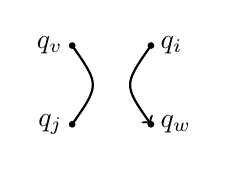
\begin{tikzpicture}[scale=0.50]
\draw[black, thick][-] (-1,-1) .. controls (-0.3,0) .. (-1,1) ;
\draw[black, thick][<-] (1,-1) .. controls (0.3,0) .. (1,1);
\filldraw[black] (-1,1) circle (2pt) node[anchor=east]{$q_{v}$};
\filldraw[black] (1,1) circle (2pt) node[anchor=west]{$q_{i}$};
\filldraw[black] (-1,-1) circle (2pt) node[anchor=east]{$q_{j}$};
\filldraw[black] (1,-1) circle (2pt) node[anchor=west]{$q_{w}$};
\end{tikzpicture}}; & \node{}; \node {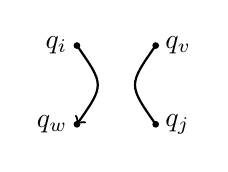
\begin{tikzpicture}[scale=0.50]
\draw[black, thick][<-] (-1,-1) .. controls (-0.3,0) .. (-1,1) ;
\draw[black, thick][-] (1,-1) .. controls (0.3,0) .. (1,1);
\filldraw[black] (-1,1) circle (2pt) node[anchor=east]{$q_{i}$};
\filldraw[black] (1,1) circle (2pt) node[anchor=west]{$q_{v}$};
\filldraw[black] (-1,-1) circle (2pt) node[anchor=east]{$q_{w}$};
\filldraw[black] (1,-1) circle (2pt) node[anchor=west]{$q_{j}$};
\end{tikzpicture}}; & \node {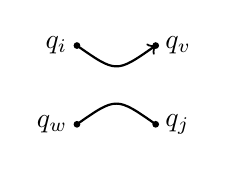
\begin{tikzpicture}[scale=0.50]
\draw[black, thick][->] (-1,1) .. controls (0,0.3) .. (1,1) ;
\draw[black, thick] (-1,-1) .. controls (0,-0.3) .. (1,-1);
\filldraw[black] (-1,1) circle (2pt) node[anchor=east]{$q_{i}$};
\filldraw[black] (1,1) circle (2pt) node[anchor=west]{$q_{v}$};
\filldraw[black] (-1,-1) circle (2pt) node[anchor=east]{$q_{w}$};
\filldraw[black] (1,-1) circle (2pt) node[anchor=west]{$q_{j}$};
\end{tikzpicture}}; \\
};
\end{tikzpicture}
\caption{The 1-smoothing (left) and the 0-smoothing (right) of a crossing}
\label{fig3}
\end{figure}

Applying one of the two resolutions at every crossing of the diagram $\mathcal{D}$, we are left with a disjoint union of circles (an unlink diagram) that we call a \textbf{smoothing} of $\mathcal{D}$. A $k$-crossing diagram has $2^{k}$ smoothings, labeled by words $\mathbf{v}\in \{0,1\}^{k}$. Here $\mathbf{v}_{l}=1$ (resp. $\mathbf{v}_{l}=0$) if at the $l$-th crossing, the 1-smoothing (resp. the 0-smoothing) has been applied.

\begin{figure}[H] 
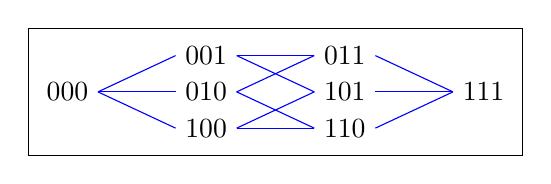
\begin{tikzpicture}
\matrix [draw,column sep={1cm}]
{
\node {}; & \node (a) {$001$}; & \node (b) {$011$}; & \node{};\\
\node (c) {$000$}; & \node (d) {$010$}; & \node (e) {$101$}; & \node (f) {$111$};\\
\node {}; & \node (g) {$100$}; & \node (h) {$110$}; & \node{};\\
};
\draw [blue] (a.east) -- (b.west) node [above,midway] {};
\draw [blue] (a.east) -- (e.west) node [above,midway] {};
\draw [blue] (c.east) -- (a.west) node [above,midway] {};
\draw [blue] (c.east) -- (d.west) node [above,midway] {};
\draw [blue] (c.east) -- (g.west) node [above,midway] {};
\draw [blue] (d.east) -- (b.west) node [above,midway] {};
\draw [blue] (d.east) -- (h.west) node [above,midway] {};
\draw [blue] (g.east) -- (e.west) node [above,midway] {};
\draw [blue] (e.east) -- (f.west) node [above,midway] {};
\draw [blue] (b.east) -- (f.west) node [above,midway] {};
\draw [blue] (h.east) -- (f.west) node [above,midway] {};
\draw [blue] (g.east) -- (h.west) node [above,midway] {};
\end{tikzpicture}
\caption{The cube of smoothings for a diagram with 3 crossings}
\label{fig4}
\end{figure}

The set $\{0,1\}^{k}$  is the vertex set of a $k$-dimensional hypercube, with edges between every two words that differ exactly at one place. We draw the cube in a skewered manner, so that all vertices whose sum of coordinates equals $i$ have the same $x$-coordinate $i-k_{-}$ (see Figure \ref{fig4}). Let $\Gamma _{\mathbf{v}}$ denote the smoothing labeled by a word $\mathbf{v}$, and let $c_{\mathbf{v}}$ denote the number of components of $\Gamma _{\mathbf{v}}$. Denote by $r_{\mathbf{v}}$ the number of $1$'s in the word $\mathbf{v}$. The unnormalised Jones polynomial of the link with a diagram $\mathcal{D}$ is given by $$\widehat{J}(\mathcal{D})(q)=\sum _{\mathbf{v}\in \{0,1\}^{k}}(-1)^{r_{\mathbf{v}}+k_{-}}\,q^{r_{\mathbf{v}}+k_{+}-2k_{-}}\left (q+q^{-1}\right )^{c_{\mathbf{v}}}\;.$$ The ``usual'' Jones polynomial may be obtained from the Jones polynomial $J(\mathcal{D})(q)=\frac{\widehat{J}(\mathcal{D})(q)}{q+q^{-1}}$ by the substitution $q=-t^{\frac{1}{2}}$.

An edge between two vertices in the cube of smoothings is usually labelled by a word of ones and zeroes with a star at the position where the two vertices differ. Thus for example the edge joining the vertex $010$ and $011$ is labeled by $01\star$. Every edge is oriented as an arrow from the vertex with $\star =0$ to the vertex with $\star =1$. The smoothings labelled by two adjacent vertices $\mathbf{v}\stackrel{\zeta }{\to}\mathbf{v}'$ only differ inside the region of a small disc (the changing disc) around the crossing, corresponding to the $\star $ in $\zeta $, where the $0$-smoothing switches to $1$-smoothing. The edge $\zeta $ corresponds to a cobordism $W_{\zeta }$ between the smoothings. Outside the changing disc, this cobordism is just a product of $\Gamma _{\mathbf{v}}$ with an interval, while inside the tube above the changing disc, the surface looks like a saddle between the two resolutions. 

We briefly recall the definition of the Khovanov complex $C^{\ast ,\ast}(\mathcal{D})$ of an oriented link diagram $\mathcal{D}$. Denote by $X$ a graded $\mathbb{Q}$-vector space with two basis elements $x_{+}$ and $x_{-}$, such that $\deg (x_{+})=1$ and $\deg (x_{-})=-1$. To each word $\mathbf{v}\in \{0,1\}$ we associate the vector space $$X_{\mathbf{v}}=X^{\otimes c_{\mathbf{v}}}\{r_{\mathbf{v}}+k_{+}-2k_{-}\}\;,$$ where $F\{m\}$ denotes the grading shift that lowers gradings of all elements in a graded vector space $F$ by an integer $m$. Then define $$C^{i,\ast }(\mathcal{D})=\oplus _{\stackrel{\mathbf{v}\in \{0,1\}^{k}}{r_{\mathbf{v}}=i+k_{-}}}X_{\mathbf{v}}\;.$$ 
Thus, every smoothing $\Gamma _{\mathbf{v}}$ in the cube of smoothings has an associated graded vector space $X_{\mathbf{v}}$; and the space $C^{i,\ast}(\mathcal{D})$ is the direct sum of all vector spaces in the column $i+k_{-}$ of the cube. Every element of $C^{i,j}(\mathcal{D})$ has two gradings: the \textbf{homological grading} $i$ and the $q$-\textbf{grading} $j$. If $c\in C^{i,j}(\mathcal{D})$ is an element whose degree in $X_{\mathbf{v}}$ equals $\deg (c)$, then $i=r_{\mathbf{v}}-k_{-}$  and $j=\deg(c)+i+k_{+}-k_{-}$. 

To every smoothing $\Gamma _{v}$ inside the cube of smoothings, we have associated the vector space $X_{\mathbf{v}}$. To a cobordism $W_{\zeta }$, corresponding to an edge $\mathbf{v}\stackrel{\zeta}{\rightarrow}\mathbf{v}'$, we associate a linear map $d_{\zeta }\colon X_{\mathbf{v}}\to X_{\mathbf{v}'}$. This map restricts to the identity map for any part of $W_{\zeta}$ that is a trivial (product) cobordism, while a pair of pants surface (a cobordism between one circle and a pair of circles in either order) gives rise to two linear maps $m\colon X\otimes X\to X$ and $\Delta \colon X\to X\otimes X$. These are defined by 
\begin{xalignat*}{1}
& m(x_{+}\otimes x_{+})=x_{+}\,,\quad m(x_{+}\otimes x_{-})=m(x_{-}\otimes x_{+})=x_{-}\,,\quad m(x_{-}\oplus x_{-})=0,\\
& \Delta (x_{+})=x_{-}\otimes x_{+}+x_{+}\otimes x_{-}\,,\quad m(x_{-})=x_{-}\otimes x_{-}\;.
\end{xalignat*}  
Every edge $\zeta $ in the cube of smoothings has a sign, given by $$\textrm{sign}(\zeta)=(-1)^{\textrm{number of 1's to the left of $\star$ in $\zeta$}}\;.$$ To define the differential $d^{i}\colon C^{i,\ast}(\mathcal{D})\to C^{i+1,\ast}(\mathcal{D})$, we set $$d^{i}(c)=\sum _{Tail (\zeta )=\mathbf{v}}\textrm{sign}(\zeta )d_{\zeta }(c)$$
for any $c\in X_{\mathbf{v}}\subset C^{i,\ast}(\mathcal{D})$, and extend by linearity. The \textbf{Khovanov homology} of an oriented link diagram $\mathcal{D}$ is the homology of this complex: $$KH^{\ast ,\ast}(\mathcal{D})=H(C^{\ast ,\ast}\left (\mathcal{D}),d\right )\;.$$ It turns out this homology is a fine knot and link invariant. Its Euler characteristic is precisely the unnormalised Jones polynomial, as the following proposition states:

\begin{proposition} For any link diagram $\mathcal{D}$, we have $\sum (-1)^{i}qdim(KH^{i,\ast}(\mathcal{D}))=\widehat{J}(\mathcal{D})$. 
\end{proposition}



\subsection{The cube of polygonal smoothings}

Let $\mathcal{D}$ be a polygonal link diagram with a labeled set of vertices $\{q_{1},q_{2},\ldots ,q_{n}\}$. $\mathcal{D}$ has a decomposition as a union of projections of link components. Two vertices are called \textbf{$c$-adjacent} if they belong to the projection of a component $c$ and they are connected by an edge of the diagram. A permutation $\sigma \in S_{n}$ \textbf{preserves} the diagram $\mathcal{D}$ if for every $i,j\in \{1,2,\ldots n\}$ and every component $c$ of $\mathcal{D}$ we have $$q_{i}\textrm{ and $q_{j}$ are $c$-adjacent} \Leftrightarrow q_{\sigma (i)}\textrm{ and $q_{\sigma (j)}$ are $c$-adjacent}\;.$$
Thus, such permutation preserves both the decomposition of $\mathcal{D}$ into link components and the adjacency of vertices. The \textbf{group of the diagram} $\mathcal{D}$ is the subgroup $G_{\mathcal{D}}$ of $S_n$ that contains all the permutations preserving $\mathcal{D}$. It follows that $G_{\mathcal{D}}$ is a direct product of dihedral groups, corresponding to the connected components of the underlying link. We enumerate the components of $\mathcal{D}$ (and their corresponding factors in $G_{\mathcal{D}}$) with respect to the lowest index of their vertices (thus the first component contains the vertex $q_1$, the second component contains the vertex with the lowest index not contained in the first component, etc.). The factor of $G_{\mathcal{D}}$, corresponding to the $i$-th component of $\mathcal{D}$, will be denoted by $G_{\mathcal{D}}^{(i)}$.\\ 

Consider a good link diagram $$\mathcal{D}=\left ((q_{n_0+1},\ldots ,q_{n_{1}}),(q_{n_{1}+1},\ldots ,q_{n_{2}}),\ldots (q_{n_{r-1}+1},\ldots ,q_{n_r})\right )$$ with crossings $\{\overline{q_{i_l}q_{j_{l}}}\cap \overline{q_{v_l}q_{w_{l}}}\colon l=1,2,\ldots ,k\}$. Denote by $\epsilon _{l}\in \{-1,1\}$ the sign of the $l$-th crossing. We choose a notation for various (partial) smoothings of the diagram $\mathcal{D}$. For any vector $\mathbf{v}\in \{0,1,2\}^{k}$, denote by $\mathcal{D}_{\mathbf{v}}$ the diagram obtained from $\mathcal{D}$ by \begin{itemize}
\item $0$-smoothing the $l$-th crossing if $\mathbf{v}_{l}=0$, 
\item $1$-smoothing the $l$-th crossing if $\mathbf{v}_{l}=1$ and
\item leaving the $l$-th crossing as it is if $\mathbf{v}_{l}=2$. 
\end{itemize}
Every (partial) smoothing is given by a graph $\Gamma _{\mathbf{v}}$ on the fixed set of vertices $\{q_{1},q_{2},\ldots ,q_{n}\}$, that may also be considered as a link diagram. We will denote by $G_{\mathbf{v}}=G_{\Gamma _{\mathbf{v}}}$ the group of this diagram. We would like to choose a set of generators of $G_{\mathbf{v}}$ in a systematic fashion. \\

Each crossing of our link diagram gives rise to certain reflections in the cube of smoothings. Suppose that two vertices $q_a$ and $q_b$ correspond to the $i$-th component of $\Gamma _{\mathbf{v}}$. Then we denote by $\xi _{\mathbf{v},a,b}\in G_{\mathbf{v}}^{(i)}$ the order $2$ permutation that corresponds to the reflection interchanging $q_a$ and $q_{b}$ (i.e. a product of disjoint transpositions, one of which is the transposition $\cycle{a,b}$, as an element of the corresponding dihedral group). \\

A smoothing of an oriented link diagram does not, by itself, have a uniquely defined orientation. However, a chosen orientation of a partial smoothing may induce an orientation of its ``smoothing ancestor''. Let $\mathbf{v},\mathbf{v}'\in \{0,1,2\}^{k}$ be any two vectors with $\mathbf{v}_{m}=2$, $\mathbf{v}'_{m}\neq 2$ and $\mathbf{v}_{l}=\mathbf{v}'_{l}$ for $l\neq m$. Given an orientation of the partial smoothing $\Gamma _{\mathbf{v}}$, its \textbf{induced orientation} on $\Gamma _{\mathbf{v}'}$ is defined as follows: \begin{itemize}
\item $i_m$ should be the starting index of one of the new edges produced in this smoothing.
\item  If the vertices $q_{i_m}$ and $q_{v_m}$ do not belong to the same component of $\Gamma _{\mathbf{v}'}$, then $v_m$ is the starting index of one of the new edges produced in this smoothing, see Figure \ref{fig3}. 
\item The orientation of any component of $\Gamma _{\mathbf{v}'}$ that contains neither $q_{i_{m}}$ nor $q_{v_{m}}$ stays the same as in $\Gamma _{\mathbf{v}}$. 
\end{itemize}

Fixing an orientation $\omega $ of a partial smoothing $\Gamma _{\mathbf{v}}$, let us denote by $\lambda _{\mathbf{v},i}^{\omega }\in G_{\mathbf{v}}^{(i)}$ the cyclic permutation that maps each vertex of the $i$-th component of the smoothing $\Gamma _{\mathbf{v}}$ to its following $c$-adjacent vertex with respect to the orientation $\omega $. The cyclic permutation $\lambda _{\mathbf{v},i}^{\omega }$, corresponding to the component of $\Gamma _{\mathbf{v}}$ that contains two vertices $q_{a}, q_{b}$, will sometimes be denoted by $\lambda _{\mathbf{v},a,b}^{\omega }$. Moreover, we define $\sigma _{\mathbf{v}}^{\omega }=\prod _{i=1}^{c_{\mathbf{v}}}\lambda _{\mathbf{v},i}^{\omega }\in G_{\mathbf{v}}$. We will call $\sigma _{\mathbf{v}}^{\omega}$ the \textbf{permutation of the smoothing} $\Gamma _{\mathbf{v}}$ with orientation $\omega $. To simplify notation, we will sometimes omit the superscript that refers to the orientation. 

\begin{remark} Observe that the subgroup $G_{\mathbf{v}}^{(i)}\leq S_{n}$ is completely determined by the ele\-ment $\lambda _{\mathbf{v},i}^{\omega }$. Indeed, if $\lambda _{\mathbf{v},i}^{\omega }$ is given by the cyclic permutation $\cycle{c_{1},c_{2},\ldots ,c_{d}}\in S_{n}$, then the order $2$ generator of the dihedral group $G_{\mathbf{v}}^{(i)}\cong D_{d}$ can be chosen as the involution $\cycle{c_{1},c_{d}}\cycle{c_{2},c_{d-1}}\ldots \cycle{c_{\frac{d}{2}},c_{\frac{d+2}{2}}}$ if $d$ is even or $\cycle{c_{1},c_{d}}\cycle{c_{2},c_{d-1}}\ldots \cycle{c_{\frac{d-1}{2}},c_{\frac{d+3}{2}}}$ if $d$ is odd. It follows that $\sigma _{\mathbf{v}}^{\omega }$, the permutation of a smoothing, uniquely determines $G_{\mathbf{v}}$, the group of the diagram $\Gamma _{\mathbf{v}}$.
\end{remark}

\begin{example} Figure \ref{fig5} shows the diagram of a Whitehead link and its smoothing, labelled by the smoothing word $11011$. The initial permutation of the vertex indices is given as $\cycle{1,2,3,4,5,6,7,8}\cycle{9,10,11,12}$. The symmetry group of the smoothing $G_{11011}\cong D_{9}\times D_{3}\leq S_{12}$ is generated by $\lambda _{11011,1}=\cycle{1,9,3,8,10,5,6,12,2}$, $\lambda _{11011,2}=\cycle{7,4,11}$, $\xi _{11011,3,8}=\cycle{3,8}\cycle{9,10}\cycle{1,5}\cycle{2,6}$ and $\xi _{11011,4,7}=\cycle{4,7}$. Also, we have $\sigma _{11011}=\cycle{1,9,3,8,10,5,6,12,2}\cycle{7,4,11}$. 
\begin{figure}[H]
\begin{tikzpicture}
\matrix [draw,column sep={1cm}]
{
\node{\begin{tikzpicture}[scale=0.45]
\draw[black, thick](-6,-3) -- (-6,3);
\draw[black, thick] (-6,3) -- (-1.85,1.38);
\draw[black, thick](-1.5,1.24) -- (-1,1);
\draw[black, thick](-1,1) -- (1,-1);
\draw[black, thick](1,-1) -- (1.5,-1.2);
\draw[black, thick](1.9,-1.35) -- (6,-3);
\draw[black, thick](6,-3) -- (6,3);
\draw[black, thick](6,3) -- (1,1);
\draw[black, thick](1,1) -- (0.2,0.2);
\draw[black, thick](-0.1,-0.1) -- (-1,-1);
\draw[black, thick](-1,-1) -- (-6,-3);
\draw[black, thick](-3,0) -- (0,3);
\draw[black, thick](0,3) -- (1.6,1.4);
\draw[black, thick](1.8,1.2) -- (3,0);
\draw[black, thick](3,0) -- (0,-3);
\draw[black, thick](0,-3) -- (-1.6,-1.4);
\draw[black, thick](-1.8,-1.2) -- (-3,0);
\filldraw[black] (-6,-3) circle (2pt) node[anchor=east]{$1$};
\filldraw[black] (-6,3) circle (2pt) node[anchor=east]{$2$};
\filldraw[black] (-1,1) circle (2pt) node[anchor=west]{$3$};
\filldraw[black] (1,-1) circle (2pt) node[anchor=north]{$4$};
\filldraw[black] (6,-3) circle (2pt) node[anchor=west]{$5$};
\filldraw[black] (6,3) circle (2pt) node[anchor=west]{$6$};
\filldraw[black] (1,1) circle (2pt) node[anchor=east]{$7$};
\filldraw[black] (-1,-1) circle (2pt) node[anchor=north]{$8$};
\filldraw[black] (-3,0) circle (2pt) node[anchor=east]{$9$};
\filldraw[black] (0,-3) circle (2pt) node[anchor=north]{$10$};
\filldraw[black] (3,0) circle (2pt) node[anchor=west]{$11$};
\filldraw[black] (0,3) circle (2pt) node[anchor=south]{$12$};
\end{tikzpicture}}; & \node{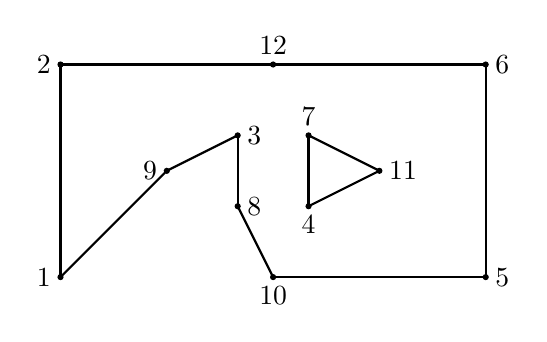
\begin{tikzpicture}[scale=0.45]
\draw[black, thick](-6,-3) -- (-6,3);
\draw[black, thick] (-6,3) -- (0,3);
\draw[black, thick](0,3) -- (6,3);
\draw[black, thick](6,3) -- (6,-3);
\draw[black, thick](6,-3) -- (0,-3);
\draw[black, thick](1,1) -- (1,-1);
\draw[black, thick](-1,1) -- (-3,0);
\draw[black, thick](-3,0) -- (-6,-3);
\draw[black, thick](-1,1) -- (-1,-1);
\draw[black, thick](-1,-1) -- (0,-3);
\draw[black, thick](1,-1) -- (3,0);
\draw[black, thick](3,0) -- (1,1);
\filldraw[black] (-6,-3) circle (2pt) node[anchor=east]{$1$};
\filldraw[black] (-6,3) circle (2pt) node[anchor=east]{$2$};
\filldraw[black] (-1,1) circle (2pt) node[anchor=west]{$3$};
\filldraw[black] (1,-1) circle (2pt) node[anchor=north]{$4$};
\filldraw[black] (6,-3) circle (2pt) node[anchor=west]{$5$};
\filldraw[black] (6,3) circle (2pt) node[anchor=west]{$6$};
\filldraw[black] (1,1) circle (2pt) node[anchor=south]{$7$};
\filldraw[black] (-1,-1) circle (2pt) node[anchor=west]{$8$};
\filldraw[black] (-3,0) circle (2pt) node[anchor=east]{$9$};
\filldraw[black] (0,-3) circle (2pt) node[anchor=north]{$10$};
\filldraw[black] (3,0) circle (2pt) node[anchor=west]{$11$};
\filldraw[black] (0,3) circle (2pt) node[anchor=south]{$12$};
\end{tikzpicture}};\\
};
\end{tikzpicture}
\caption{A labeled polygonal link and one of its smoothings}
\label{fig5}
\end{figure}
\end{example}

\begin{example} \label{ex1} Figure \ref{fig1} shows a good diagram of a polygonal trefoil knot with nine vertices. Indices of the crossing vertices are given as $i_{1}=3$, $j_{1}=4$, $v_{1}=8$, $w_{1}=9$, $i_{2}=6$, $j_{2}=7$, $v_{2}=2$, $w_{2}=3$, $i_{3}=9$, $j_{3}=1$, $v_{3}=5$, $w_{3}=6$. The cube of smoothings for this diagram is given in Figure \ref{fig7}, and its cube of permutations $\sigma _{\mathbf{v}}$ is given in Figure \ref{fig15}.  
\end{example}


\begin{landscape}
\thispagestyle{empty}
\begin{figure}
\begin{center}
\caption{The cube of smoothings for a trefoil}
\label{fig7}
\begin{tikzpicture}
\matrix [draw,column sep={1cm}]
{
\node {}; & \node (a) {\begin{tikzpicture}[scale=0.70]
\draw[black, thick](-1,2) -- (-2,0);
\draw[black, thick](2,0) -- (1,2);
\draw[black, thick](1,2) -- (-1,2);
\draw[black, thick](-0.5,0.5) -- (0.5,0.5);
\draw[black, thick](-0.5,0.5) -- (0,-1);
\draw[black, thick](-1,-2) -- (1,-2);
\draw[black, thick](2,0) -- (0.5,0.5);
\draw[black, thick](1,-2) -- (0,-1);
\draw[black, thick](-2,0) -- (-1,-2);
\filldraw[black] (-1,2) circle (2pt) node[anchor=south]{$7$};
\filldraw[black] (-2,0) circle (2pt) node[anchor=east]{$8$};
\filldraw[black] (0,-1) circle (2pt) node[anchor=west]{$9$};
\filldraw[black] (2,0) circle (2pt) node[anchor=west]{$1$};
\filldraw[black] (1,2) circle (2pt) node[anchor=south]{$2$};
\filldraw[black] (-0.5,0.5) circle (2pt) node[anchor=south]{$3$};
\filldraw[black] (-1,-2) circle (2pt) node[anchor=east]{$4$};
\filldraw[black] (1,-2) circle (2pt) node[anchor=west]{$5$};
\filldraw[black] (0.5,0.5) circle (2pt) node[anchor=south]{$6$};
\end{tikzpicture}}; & \node (b) {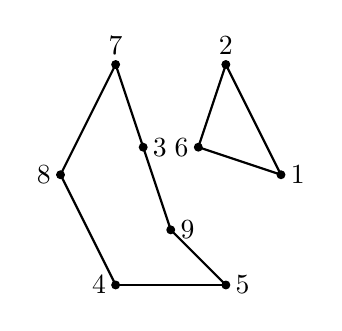
\begin{tikzpicture}[scale=0.70]
\draw[black, thick](-1,2) -- (-2,0);
\draw[black, thick](2,0) -- (1,2);
\draw[black, thick](1,2) -- (0.5,0.5);
\draw[black, thick](-0.5,0.5) -- (-1,2);
\draw[black, thick](-0.5,0.5) -- (0,-1);
\draw[black, thick](-1,-2) -- (-2,0);
\draw[black, thick](0.5,0.5) -- (2,0);
\draw[black, thick](-1,-2) -- (1,-2);
\draw[black, thick](0,-1) -- (1,-2);
\filldraw[black] (-1,2) circle (2pt) node[anchor=south]{$7$};
\filldraw[black] (-2,0) circle (2pt) node[anchor=east]{$8$};
\filldraw[black] (0,-1) circle (2pt) node[anchor=west]{$9$};
\filldraw[black] (2,0) circle (2pt) node[anchor=west]{$1$};
\filldraw[black] (1,2) circle (2pt) node[anchor=south]{$2$};
\filldraw[black] (-0.5,0.5) circle (2pt) node[anchor=west]{$3$};
\filldraw[black] (-1,-2) circle (2pt) node[anchor=east]{$4$};
\filldraw[black] (1,-2) circle (2pt) node[anchor=west]{$5$};
\filldraw[black] (0.5,0.5) circle (2pt) node[anchor=east]{$6$};
\end{tikzpicture}}; & \node{};\\
\node (c) {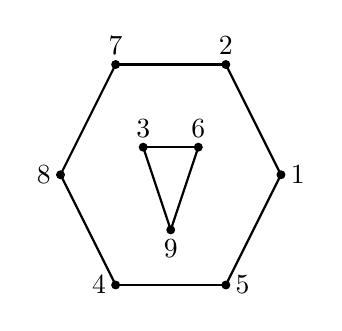
\begin{tikzpicture}[scale=0.70]
\draw[black, thick](-1,2) -- (-2,0);
\draw[black, thick](2,0) -- (1,2);
\draw[black, thick](-1,2) -- (1,2);
\draw[black, thick](-0.5,0.5) -- (0.5,0.5);
\draw[black, thick](-1,-2) -- (-2,0);
\draw[black, thick](0.5,0.5) -- (0,-1);
\draw[black, thick](-1,-2) -- (1,-2);
\draw[black, thick](2,0) -- (1,-2);
\draw[black, thick](0,-1) -- (-0.5,0.5);
\filldraw[black] (-1,2) circle (2pt) node[anchor=south]{$7$};
\filldraw[black] (-2,0) circle (2pt) node[anchor=east]{$8$};
\filldraw[black] (0,-1) circle (2pt) node[anchor=north]{$9$};
\filldraw[black] (2,0) circle (2pt) node[anchor=west]{$1$};
\filldraw[black] (1,2) circle (2pt) node[anchor=south]{$2$};
\filldraw[black] (-0.5,0.5) circle (2pt) node[anchor=south]{$3$};
\filldraw[black] (-1,-2) circle (2pt) node[anchor=east]{$4$};
\filldraw[black] (1,-2) circle (2pt) node[anchor=west]{$5$};
\filldraw[black] (0.5,0.5) circle (2pt) node[anchor=south]{$6$};
\end{tikzpicture}}; & \node (d) {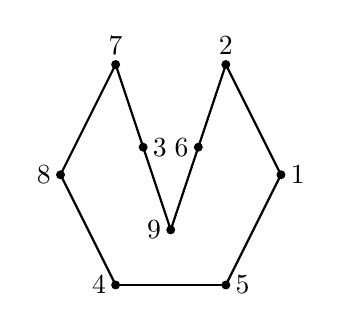
\begin{tikzpicture}[scale=0.70]
\draw[black, thick](-1,2) -- (-2,0);
\draw[black, thick](2,0) -- (1,2);
\draw[black, thick](1,2) -- (0.5,0.5);
\draw[black, thick](-0.5,0.5) -- (-1,2);
\draw[black, thick](-1,-2) -- (-2,0);
\draw[black, thick](0.5,0.5) -- (0,-1);
\draw[black, thick](-1,-2) -- (1,-2);
\draw[black, thick](2,0) -- (1,-2);
\draw[black, thick](0,-1) -- (-0.5,0.5);
\filldraw[black] (-1,2) circle (2pt) node[anchor=south]{$7$};
\filldraw[black] (-2,0) circle (2pt) node[anchor=east]{$8$};
\filldraw[black] (0,-1) circle (2pt) node[anchor=east]{$9$};
\filldraw[black] (2,0) circle (2pt) node[anchor=west]{$1$};
\filldraw[black] (1,2) circle (2pt) node[anchor=south]{$2$};
\filldraw[black] (-0.5,0.5) circle (2pt) node[anchor=west]{$3$};
\filldraw[black] (-1,-2) circle (2pt) node[anchor=east]{$4$};
\filldraw[black] (1,-2) circle (2pt) node[anchor=west]{$5$};
\filldraw[black] (0.5,0.5) circle (2pt) node[anchor=east]{$6$};
\end{tikzpicture}}; & \node (e) {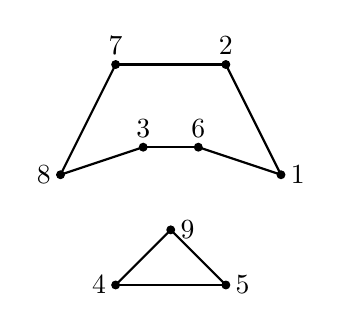
\begin{tikzpicture}[scale=0.70]
\draw[black, thick](-1,2) -- (-2,0);
\draw[black, thick](2,0) -- (1,2);
\draw[black, thick](1,2) -- (-1,2);
\draw[black, thick](-0.5,0.5) -- (0.5,0.5);
\draw[black, thick](-0.5,0.5) -- (-2,0);
\draw[black, thick](-1,-2) -- (1,-2);
\draw[black, thick](2,0) -- (0.5,0.5);
\draw[black, thick](1,-2) -- (0,-1);
\draw[black, thick](0,-1) -- (-1,-2);
\filldraw[black] (-1,2) circle (2pt) node[anchor=south]{$7$};
\filldraw[black] (-2,0) circle (2pt) node[anchor=east]{$8$};
\filldraw[black] (0,-1) circle (2pt) node[anchor=west]{$9$};
\filldraw[black] (2,0) circle (2pt) node[anchor=west]{$1$};
\filldraw[black] (1,2) circle (2pt) node[anchor=south]{$2$};
\filldraw[black] (-0.5,0.5) circle (2pt) node[anchor=south]{$3$};
\filldraw[black] (-1,-2) circle (2pt) node[anchor=east]{$4$};
\filldraw[black] (1,-2) circle (2pt) node[anchor=west]{$5$};
\filldraw[black] (0.5,0.5) circle (2pt) node[anchor=south]{$6$};
\end{tikzpicture}}; & \node (f) {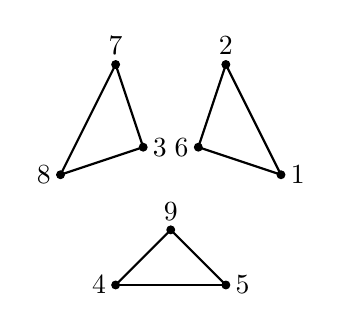
\begin{tikzpicture}[scale=0.70]
\draw[black, thick](-1,2) -- (-2,0);
\draw[black, thick](2,0) -- (1,2);
\draw[black, thick](1,2) -- (0.5,0.5);
\draw[black, thick](-0.5,0.5) -- (-1,2);
\draw[black, thick](-0.5,0.5) -- (-2,0);
\draw[black, thick](0.5,0.5) -- (2,0);
\draw[black, thick](-1,-2) -- (1,-2);
\draw[black, thick](0,-1) -- (1,-2);
\draw[black, thick](0,-1) -- (-1,-2);
\filldraw[black] (-1,2) circle (2pt) node[anchor=south]{$7$};
\filldraw[black] (-2,0) circle (2pt) node[anchor=east]{$8$};
\filldraw[black] (0,-1) circle (2pt) node[anchor=south]{$9$};
\filldraw[black] (2,0) circle (2pt) node[anchor=west]{$1$};
\filldraw[black] (1,2) circle (2pt) node[anchor=south]{$2$};
\filldraw[black] (-0.5,0.5) circle (2pt) node[anchor=west]{$3$};
\filldraw[black] (-1,-2) circle (2pt) node[anchor=east]{$4$};
\filldraw[black] (1,-2) circle (2pt) node[anchor=west]{$5$};
\filldraw[black] (0.5,0.5) circle (2pt) node[anchor=east]{$6$};
\end{tikzpicture}};\\
\node {}; & \node (g) {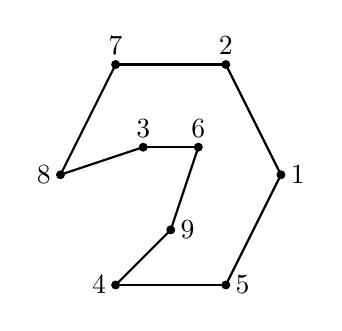
\begin{tikzpicture}[scale=0.70]
\draw[black, thick](-1,2) -- (-2,0);
\draw[black, thick](2,0) -- (1,2);
\draw[black, thick](1,2) -- (-1,2);
\draw[black, thick](-0.5,0.5) -- (0.5,0.5);
\draw[black, thick](-0.5,0.5) -- (-2,0);
\draw[black, thick](-1,-2) -- (1,-2);
\draw[black, thick](0,-1) -- (0.5,0.5);
\draw[black, thick](1,-2) -- (2,0);
\draw[black, thick](0,-1) -- (-1,-2);
\filldraw[black] (-1,2) circle (2pt) node[anchor=south]{$7$};
\filldraw[black] (-2,0) circle (2pt) node[anchor=east]{$8$};
\filldraw[black] (0,-1) circle (2pt) node[anchor=west]{$9$};
\filldraw[black] (2,0) circle (2pt) node[anchor=west]{$1$};
\filldraw[black] (1,2) circle (2pt) node[anchor=south]{$2$};
\filldraw[black] (-0.5,0.5) circle (2pt) node[anchor=south]{$3$};
\filldraw[black] (-1,-2) circle (2pt) node[anchor=east]{$4$};
\filldraw[black] (1,-2) circle (2pt) node[anchor=west]{$5$};
\filldraw[black] (0.5,0.5) circle (2pt) node[anchor=south]{$6$};
\end{tikzpicture}}; & \node (h) {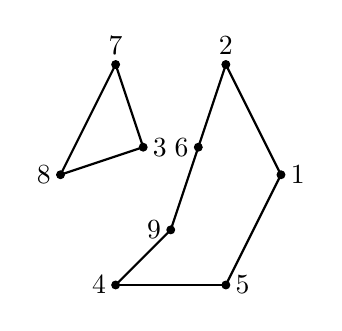
\begin{tikzpicture}[scale=0.70]
\draw[black, thick](-1,2) -- (-2,0);
\draw[black, thick](2,0) -- (1,2);
\draw[black, thick](1,2) -- (0.5,0.5);
\draw[black, thick](-0.5,0.5) -- (-1,2);
\draw[black, thick](-0.5,0.5) -- (-2,0);
\draw[black, thick](0.5,0.5) -- (0,-1);
\draw[black, thick](-1,-2) -- (1,-2);
\draw[black, thick](2,0) -- (1,-2);
\draw[black, thick](0,-1) -- (-1,-2);
\filldraw[black] (-1,2) circle (2pt) node[anchor=south]{$7$};
\filldraw[black] (-2,0) circle (2pt) node[anchor=east]{$8$};
\filldraw[black] (0,-1) circle (2pt) node[anchor=east]{$9$};
\filldraw[black] (2,0) circle (2pt) node[anchor=west]{$1$};
\filldraw[black] (1,2) circle (2pt) node[anchor=south]{$2$};
\filldraw[black] (-0.5,0.5) circle (2pt) node[anchor=west]{$3$};
\filldraw[black] (-1,-2) circle (2pt) node[anchor=east]{$4$};
\filldraw[black] (1,-2) circle (2pt) node[anchor=west]{$5$};
\filldraw[black] (0.5,0.5) circle (2pt) node[anchor=east]{$6$};
\end{tikzpicture}};  & \node{};\\
};
\draw [->,blue,thick] (a.east) -- (b.west) node [above,midway] {};
\draw [->,blue,thick] (a.east) -- (e.west) node [above,midway] {};
\draw [->,blue,thick] (c.east) -- (a.west) node [above,midway] {};
\draw [->,blue,thick] (c.east) -- (d.west) node [above,midway] {};
\draw [->,blue,thick] (c.east) -- (g.west) node [above,midway] {};
\draw [->,red,thick] (d.east) -- (b.west) node [above,midway] {};
\draw [->,blue,thick] (d.east) -- (h.west) node [above,midway] {};
\draw [->,red,thick] (g.east) -- (e.west) node [above,midway] {};
\draw [->,red,thick] (e.east) -- (f.west) node [above,midway] {};
\draw [->,blue,thick] (b.east) -- (f.west) node [above,midway] {};
\draw [->,blue,thick] (h.east) -- (f.west) node [above,midway] {};
\draw [->,red,thick] (g.east) -- (h.west) node [above,midway] {};
\end{tikzpicture}
\end{center}
\end{figure}
\end{landscape}


\begin{figure}[H] 
\caption{The cube of permutations $\sigma _{\mathbf{v}}$ for a trefoil}
\label{fig15}
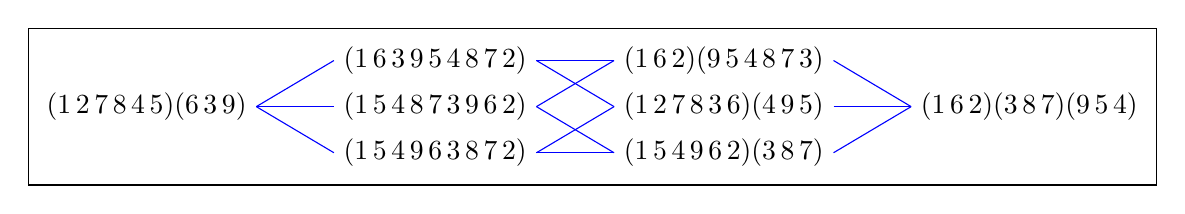
\begin{tikzpicture}
\matrix [draw,column sep={1cm}]
{
\node {}; & \node (a) {$\cycle{1,6,3,9,5,4,8,7,2}$}; & \node (b) {$\cycle{1,6,2}\cycle{9,5,4,8,7,3}$}; & \node{};\\
\node (c) {$\cycle{1,2,7,8,4,5}\cycle{6,3,9}$}; & \node (d) {$\cycle{1,5,4,8,7,3,9,6,2}$}; & \node (e) {$\cycle{1,2,7,8,3,6}\cycle{4,9,5}$}; & \node (f) {$\cycle{1,6,2}\cycle{3,8,7}\cycle{9,5,4}$};\\
\node {}; & \node (g) {$\cycle{1,5,4,9,6,3,8,7,2}$}; & \node (h) {$\cycle{1,5,4,9,6,2}\cycle{3,8,7}$}; & \node{};\\
};
\draw [blue] (a.east) -- (b.west) node [above,midway] {};
\draw [blue] (a.east) -- (e.west) node [above,midway] {};
\draw [blue] (c.east) -- (a.west) node [above,midway] {};
\draw [blue] (c.east) -- (d.west) node [above,midway] {};
\draw [blue] (c.east) -- (g.west) node [above,midway] {};
\draw [blue] (d.east) -- (b.west) node [above,midway] {};
\draw [blue] (d.east) -- (h.west) node [above,midway] {};
\draw [blue] (g.east) -- (e.west) node [above,midway] {};
\draw [blue] (e.east) -- (f.west) node [above,midway] {};
\draw [blue] (b.east) -- (f.west) node [above,midway] {};
\draw [blue] (h.east) -- (f.west) node [above,midway] {};
\draw [blue] (g.east) -- (h.west) node [above,midway] {};
\end{tikzpicture}
\end{figure}


\begin{lemma} \label{lemma1} Let $\pi \in S_{n}$ be a permutation, written as a product of disjoint cycles \begin{xalignat}{1}\label{eq1}
& \pi =\cycle{c_{1},\ldots ,c_{n_{1}}}\cycle{c_{n_{1}+1},\ldots ,c_{n_{2}}}\ldots \cycle{c_{n_{r}+1},\ldots ,c_{n}}\;.\end{xalignat}  For any two distinct indices $k,l\in \{1,2,\ldots ,n\}$, the conjugation of $\pi $ with transposition $\cycle{c_{k},c_{l}}$ causes an exchange of two elements $c_k$ and $c_l$ in the product \eqref{eq1}.
\end{lemma} 
\begin{proof} This is a well-known fact about conjugation in the permutation group $S_n$. 
\end{proof}
% First suppose that $\pi =\cycle{c_{1},c_{2},\ldots ,c_{n}}\in S_{n}$ is a cyclic permutation. Then we may compute$$\cycle{c_{k},c_{l}}\cycle{c_{1},\ldots ,c_{k},\ldots ,c_{l},\ldots ,c_{n}}\cycle{c_{k},c_{l}}=\cycle{c_{1},\ldots ,c_{k-1},c_{l},c_{k+1},\ldots ,c_{l-1},c_{k}c_{l+1},\ldots ,c_{n}}\;.$$ In the general case, the computation is similar: denoting $\pi' = \cycle{c_{k},c_{l}}\pi \cycle{c_{k},c_{l}}$, we have $\pi '(c_{k-1})=c_{l}$, $\pi '(c_{l})=c_{k+1}$, $\pi '(c_{l-1})=c_k$, $\pi '(c_{k})=c_{l+1}$ and $\pi '(c_{j})=\pi (c_{j})$ for $j\in \{1,2,\ldots n\}\backslash \{k-1,k,l-1,l\}$. 



Denote by $R(\mathcal{D})=\{\mathcal{D}_{\mathbf{v}}\colon \mathbf{v}\in \{0,1,2\}^{k}\}$ the set of all diagrams of the partial resolutions of $\mathcal{D}$. To each diagram $\mathcal{D}_{\mathbf{v}}\in R(\mathcal{D})$ we can associate its group $G_{\mathbf{v}}=G_{\mathcal{D}_{\mathbf{v}}}\leq S_{n}$ and a chosen permutation $\sigma _{\mathbf{v}}\in G_{\mathbf{v}}$. For example, $$\sigma _{2^k}=\cycle{1,2,\ldots ,n_{1}}\cycle{n_{1}+1,n_{1}+2,\ldots ,n_{2}}\ldots \cycle{n_{r-1}+1,n_{r-1}+2,\ldots ,n_{r}}\;.$$ We would like to compute the permutation $\sigma _{\mathbf{v}}$, corresponding to a given diagram $\mathcal{D}_{\mathbf{v}}$. First we study the local change of the permutation when smoothing a given crossing.\\

\begin{Theorem} \label{th1} Fix an index $l\in \{1,2,\ldots ,k\}$ and let $\mathbf{v}\in \{0,1,2\}^{k}$ be any vector with $\mathbf{v}_{l}=2$. Denote by $\mathbf{v}^{+}$ (resp. $\mathbf{v}^{-}$) the vector obtained from $\mathbf{v}$ by changing $\mathbf{v}_{l}$ to $0$ (resp. 1). Choose an orientation $\omega $ of the smoothing $\Gamma _{\mathbf{v}}$ and denote by $\omega ^{+}$ (resp. $\omega ^{-}$) its induced orientations on the smoothings $\Gamma _{\mathbf{v}^{+}}$ (resp. $\Gamma _{\mathbf{v}^{-}}$). Suppose that $\sigma _{\mathbf{v}}^{\omega }(i_l)=j_{l}$ and $\sigma _{\mathbf{v}}^{\omega }(v_l)=w_{l}$.  \begin{enumerate}
\item ($\sigma _{\mathbf{v}^{\epsilon _{l}}})^{\omega ^{\epsilon _{l}}}=\cycle{j_{l},w_{l}}\sigma _{\mathbf{v}}^{\omega }$.
\item If $i_l$ and $v_l$ belong to the same cycle $\cycle{i_{l},j_{l},c_{1},c_{2},\ldots ,c_{m},v_{l},w_{l},d_{1}\ldots ,d_{g}}$ of $\sigma _{\mathbf{v}}^{\omega }$, then $$(\sigma _{\mathbf{v}^{-\epsilon _{l}}})^{\omega ^{-\epsilon _{l}}}=\left (\sigma _{\mathbf{v}}^{\omega }\right )^{\xi _{\mathbf{v}^{\epsilon _{l}},j_{l},v_{l}}}\;.$$
\item If $i_l$ and $v_l$ belong to two distinct cycles $\cycle{i_{l},j_{l},d_{1},d_{2},\ldots ,d_{g}}$ and $\cycle{v_{l},w_{l},c_{1},c_{2},\ldots ,c_{m}}$ of $\sigma _{\mathbf{v}}^{\omega }$, then $$(\sigma _{\mathbf{v}^{-\epsilon _{l}}})^{\omega ^{-\epsilon _{l}}}=\left (\cycle{j_{l},w_{l}}\sigma _{\mathbf{v}}^{\omega }\right )^{\xi _{\mathbf{v},v_{l},w_{l}}}\;.$$
\end{enumerate}
\end{Theorem}
\begin{proof} We consider two possible cases with several subcases. \begin{itemize}
\item[(a)] \underline{$i_l$ and $v_{l}$ belong to the same cycle $C=\cycle{i_{l},j_{l},c_{1},c_{2},\ldots ,c_{m},v_{l},w_{l},d_{1}\ldots ,d_{g}}$ of $\sigma _{\mathbf{v}}^{\omega }$}\\
In this case, a $0$-smoothing of a positive crossing ($\sigma _{\mathbf{v}^{+}}$ if $\epsilon _{l}=1$) or a $1$-smoothing of a negative crossing ($\sigma _{\mathbf{v}^{-}}$ if $\epsilon _{l}=-1$) resolves the cycle $C$ into a product of two cycles $\cycle{j_{l},c_{1},\ldots ,c_{m},v_{l}}\cycle{w_{l},d_{1},\ldots ,d_{g},i_{l}}$. This is done by composing $\sigma _{\mathbf{v}}^{\omega }$ with a single transposition $\cycle{j_{l},w_{l}}$. \\
A $1$-smoothing of a positive crossing ($\sigma _{\mathbf{v}^{-}}$ if $\epsilon _{l}=1$) or a $0$-smoothing of a negative crossing ($\sigma _{\mathbf{v}^{+}}$ if $\epsilon _{l}=-1$) resolves the cycle $C$ into a new cycle $\cycle{i_{l},v_{l},c_{m},\ldots ,c_{1},j_{l},w_{l},d_{1},\ldots ,d_{g}}$. By Lemma \ref{lemma1}, this is achieved by the conjugation of $\sigma _{\mathbf{v}}^{\omega }$ with the product of transpositions $\cycle{j_{l},v_{l}}\cycle{c_{1},c_{m}}\ldots \cycle{c_{\lfloor\frac{m}{2}\rfloor},c_{m+1-\lfloor\frac{m}{2}\rfloor}}$. 
\begin{figure}[H]\label{fig6}
\begin{center}
\begin{tikzpicture}
\node (crossing) {\begin{tikzpicture}[scale=0.50]
\draw[black, thick][<-] (-1,-1) -- (1,1);
\draw[black, thick] (-1,1) -- (-0.1,0.1);
\draw[black, thick][->] (0.1,-0.1) -- (1,-1);
\draw[dashed][->] (-1,-1) .. controls (-6,-4) and (-6,4) ..(-1,1) ;
\draw[dashed][<-] (1,1) .. controls (6,4) and (6,-4) .. (1,-1) ;
\filldraw[black] (-1,1) circle (2pt) node[anchor=south]{$v_l$};
\filldraw[black] (1,1) circle (2pt) node[anchor=south]{$i_l$};
\filldraw[black] (-1,-1) circle (2pt) node[anchor=north]{$j_l$};
\filldraw[black] (1,-1) circle (2pt) node[anchor=north]{$w_l$};
\filldraw[black] (-3,-1.75) circle (2pt) node[anchor=north]{$c_{1}$};
\filldraw[black] (-3,1.75) circle (2pt) node[anchor=south]{$c_{m}$};
\filldraw[black] (3,-1.75) circle (2pt) node[anchor=north]{$d_{1}$};
\filldraw[black] (3,1.75) circle (2pt) node[anchor=south]{$d_{g}$};
\end{tikzpicture}}; 
\node (empty) [right=of crossing] {};
\node (negative) [above=of empty] {\begin{tikzpicture}[scale=0.50]
\draw[black, thick][<-] (-1,1) .. controls (0,0.3) .. (1,1) ;
\draw[black, thick][->] (-1,-1) .. controls (0,-0.3) .. (1,-1);
\draw[dashed][->] (-1,-1) .. controls (-6,-4) and (-6,4) ..(-1,1) ;
\draw[dashed][<-] (1,1) .. controls (6,4) and (6,-4) .. (1,-1) ;
\filldraw[black] (-1,1) circle (2pt) node[anchor=south]{$v_l$};
\filldraw[black] (1,1) circle (2pt) node[anchor=south]{$i_l$};
\filldraw[black] (-1,-1) circle (2pt) node[anchor=north]{$j_l$};
\filldraw[black] (1,-1) circle (2pt) node[anchor=north]{$w_l$};
\filldraw[black] (-3,-1.75) circle (2pt) node[anchor=north]{$c_{1}$};
\filldraw[black] (-3,1.75) circle (2pt) node[anchor=south]{$c_{m}$};
\filldraw[black] (3,-1.75) circle (2pt) node[anchor=north]{$d_{1}$};
\filldraw[black] (3,1.75) circle (2pt) node[anchor=south]{$d_{g}$};
\end{tikzpicture}}; 
\node (positive) [below=of empty] {\begin{tikzpicture}[scale=0.50]
\draw[black, thick][<-] (-1,-1) .. controls (-0.3,0) .. (-1,1) ;
\draw[black, thick][<-] (1,-1) .. controls (0.3,0) .. (1,1);
\draw[dashed][->] (-1,-1) .. controls (-6,-4) and (-6,4) ..(-1,1) ;
\draw[dashed][<-] (1,1) .. controls (6,4) and (6,-4) .. (1,-1) ;
\filldraw[black] (-1,1) circle (2pt) node[anchor=south]{$v_l$};
\filldraw[black] (1,1) circle (2pt) node[anchor=south]{$i_l$};
\filldraw[black] (-1,-1) circle (2pt) node[anchor=north]{$j_l$};
\filldraw[black] (1,-1) circle (2pt) node[anchor=north]{$w_l$};
\filldraw[black] (-3,-1.75) circle (2pt) node[anchor=north]{$c_{1}$};
\filldraw[black] (-3,1.75) circle (2pt) node[anchor=south]{$c_{m}$};
\filldraw[black] (3,-1.75) circle (2pt) node[anchor=north]{$d_{1}$};
\filldraw[black] (3,1.75) circle (2pt) node[anchor=south]{$d_{g}$};
\end{tikzpicture}}; 
\draw[->] (crossing.north) -- (negative.west);
\draw[->] (crossing.south) -- (positive.west);
\end{tikzpicture}
\caption{Case (a): a $1$-smoothing (top) and a $0$-smoothing (bottom) of a positive crossing}
\end{center}
\end{figure}
\item[(b)] \underline{$i_l$ and $v_{l}$ belong to distinct cycles $\cycle{i_{l},j_{l},d_{1},d_{2},\ldots ,d_{g}}$ and $\cycle{v_{l},w_{l},c_{1},c_{2},\ldots ,c_{m}}$ of $\sigma _{\mathbf{v}}^{\omega }$}\\
In this case, a $0$-smoothing of a positive crossing ($\sigma _{\mathbf{v}^{+}}$ if $\epsilon _{l}=1$) or a $1$-smoothing of a negative crossing ($\sigma _{\mathbf{v}^{-}}$ if $\epsilon _{l}=-1$) connects the two cycles into a single cycle $\cycle{j_{l},d_{1},\ldots ,d_{g},i_{l},w_{l},c_{1},\ldots ,c_{m},v_{l}}$. This is done by composing $\sigma _{\mathbf{v}}^{\omega }$ with a single transposition $\cycle{j_{l},w_{l}}$. \\
A $1$-smoothing of a positive crossing ($\sigma _{\mathbf{v}^{-}}$ if $\epsilon _{l}=1$) or a $0$-smoothing of a negative crossing ($\sigma _{\mathbf{v}^{+}}$ if $\epsilon _{l}=-1$) resolves the product of two cycles into a single cycle $\cycle{i_{l},v_{l},c_{m},\ldots ,c_{1},w_{l},j_{l},d_{1},\ldots ,d_{g}}$. Using Lemma \ref{lemma1}, this may be achieved by composing with the transposition $\cycle{j_{l},w_{l}}$ that merges both cycles, and then conjugating with the product of transpositions $\cycle{w_{l},v_{l}}\cycle{c_{1},c_{m}}\ldots \cycle{c_{\lfloor \frac{m}{2}\rfloor},c_{m+1-\lfloor \frac{m}{2}\rfloor }}$.   
\end{itemize}
\end{proof}
\begin{figure}[H]\label{fig8}
\begin{center}
\begin{tikzpicture}
%\node (crossing) {\begin{tikzpicture}[scale=0.50]
%\draw[black, thick][<-] (-1,-1) -- (1,1);
%\draw[black, thick] (-1,1) -- (-0.1,0.1);
%\draw[black, thick][->] (0.1,-0.1) -- (1,-1);
%\draw[dashed][->] (-1,-1) .. controls (4,-11) and (6,4) ..(1,1) ;
%\draw[dashed][->] (1,-1) .. controls (-4,-11) and (-6,4) .. (-1,1) ;
%\filldraw[black] (-1,1) circle (2pt) node[anchor=south]{$v$};
%\filldraw[black] (1,1) circle (2pt) node[anchor=south]{$i$};
%\filldraw[black] (-1,-1) circle (2pt) node[anchor=north]{$j$};
%\filldraw[black] (1,-1) circle (2pt) node[anchor=north]{$w$};
%\filldraw[black] (-0.5,-3.3) circle (2pt) node[anchor=north]{$c_{1}$};
%\filldraw[black] (-3,1.2) circle (2pt) node[anchor=south]{$c_{m}$};
%\filldraw[black] (0.5,-3.3) circle (2pt) node[anchor=north]{$d_{1}$};
%\filldraw[black] (3,1.2) circle (2pt) node[anchor=south]{$d_{g}$};
%\end{tikzpicture}}; 
\node (negative) {\begin{tikzpicture}[scale=0.50]
\draw[black, thick][<-] (-1,1) .. controls (0,0.3) .. (1,1) ;
\draw[black, thick][<-] (-1,-1) .. controls (0,-0.3) .. (1,-1);
\draw[dashed][->] (-1,-1) .. controls (4,-11) and (6,4) ..(1,1) ;
\draw[dashed][<-] (1,-1) .. controls (-4,-11) and (-6,4) .. (-1,1) ;
\filldraw[black] (-1,1) circle (2pt) node[anchor=south]{$v_l$};
\filldraw[black] (1,1) circle (2pt) node[anchor=south]{$i_l$};
\filldraw[black] (-1,-1) circle (2pt) node[anchor=north]{$j_l$};
\filldraw[black] (1,-1) circle (2pt) node[anchor=north]{$w_l$};
\filldraw[black] (-0.5,-3.3) circle (2pt) node[anchor=east]{$c_{1}$};
\filldraw[black] (-3,1.2) circle (2pt) node[anchor=south]{$c_{m}$};
\filldraw[black] (0.5,-3.3) circle (2pt) node[anchor=west]{$d_{1}$};
\filldraw[black] (3,1.2) circle (2pt) node[anchor=south]{$d_{g}$};
\end{tikzpicture}}; 
\node (positive) [right=of negative] {\begin{tikzpicture}[scale=0.50]
\draw[black, thick][<-] (-1,-1) .. controls (-0.3,0) .. (-1,1) ;
\draw[black, thick][<-] (1,-1) .. controls (0.3,0) .. (1,1);
\draw[dashed][->] (-1,-1) .. controls (4,-11) and (6,4) ..(1,1) ;
\draw[dashed][->] (1,-1) .. controls (-4,-11) and (-6,4) .. (-1,1) ;
\filldraw[black] (-1,1) circle (2pt) node[anchor=south]{$v_l$};
\filldraw[black] (1,1) circle (2pt) node[anchor=south]{$i_l$};
\filldraw[black] (-1,-1) circle (2pt) node[anchor=north]{$j_l$};
\filldraw[black] (1,-1) circle (2pt) node[anchor=north]{$w_l$};
\filldraw[black] (-0.5,-3.3) circle (2pt) node[anchor=east]{$c_{1}$};
\filldraw[black] (-3,1.2) circle (2pt) node[anchor=south]{$c_{m}$};
\filldraw[black] (0.5,-3.3) circle (2pt) node[anchor=west]{$d_{1}$};
\filldraw[black] (3,1.2) circle (2pt) node[anchor=south]{$d_{g}$};
\end{tikzpicture}}; 
%\draw[->] (crossing.west) -- (negative.east);
%\draw[->] (crossing.east) -- (positive.west);
\end{tikzpicture}
\caption{Case (b): a $1$-smoothing (left) and a $0$-smoothing (right) of a positive crossing}
\end{center}
\end{figure}



\begin{Theorem} \label{th2} Fix an index $l\in \{1,2,\ldots ,k\}$ and let $\mathbf{v}\in \{0,1,2\}^{k}$ be any vector with $\mathbf{v}_{l}=2$. Denote by $\mathbf{v}^{+}$ (resp. $\mathbf{v}^{-}$) the vector obtained from $\mathbf{v}$ by changing $\mathbf{v}_{l}$ to $0$ (resp. 1). Choose an orientation $\omega $ of the smoothing $\Gamma _{\mathbf{v}}$ and denote by $\omega ^{+}$ (resp. $\omega ^{-}$) its induced orientations on the smoothings $\Gamma _{\mathbf{v}^{+}}$ (resp. $\Gamma _{\mathbf{v}^{-}}$). Suppose that $\sigma _{\mathbf{v}}^{\omega }(i_l)=j_{l}$ and $\sigma _{\mathbf{v}}^{\omega }(w_{l})=v_{l}$.  \begin{enumerate}
\item $(\sigma _{\mathbf{v}^{-\epsilon _{l}}})^{\omega ^{-\epsilon _{l}}}=\cycle{j_{l},v_{l}}\sigma _{\mathbf{v}}^{\omega }$.
\item If $i_l$ and $v_l$ belong to the same cycle $\cycle{i_{l},j_{l},c_{1},c_{2},\ldots ,c_{m},w_{l},v_{l},d_{1}\ldots ,d_{g}}$ of $\sigma _{\mathbf{v}}^{\omega}$, then $$(\sigma _{\mathbf{v}^{\epsilon _{l}}})^{\omega ^{\epsilon _{l}}}=\left (\sigma _{\mathbf{v}}^{\omega }\right )^{\xi _{\mathbf{v}^{-\epsilon _{l}},j_{l},w_{l}}}$$
\item If $i_l$ and $v_l$ belong to two distinct cycles $\cycle{i_{l},j_{l},d_{1},d_{2},\ldots ,d_{g}}$ and $\cycle{w_{l},v_{l},c_{1},c_{2},\ldots ,c_{m}}$ of $\sigma _{\mathbf{v}}^{\omega }$, then $$(\sigma _{\mathbf{v}^{\epsilon _{l}}})^{\omega ^{\epsilon _{l}}}=\left (\cycle{j_{l},v_{l}}\sigma _{\mathbf{v}}^{\omega }\right )^{\xi _{\mathbf{v},v_{l},w_{l}}}\;.$$
\end{enumerate}
\end{Theorem}
\begin{proof} We consider two possible cases with several subcases. \begin{itemize}
\item[(a)] \underline{$i_l$ and $v_{l}$ belong to the same cycle $C=\cycle{i_{l},j_{l},c_{1},c_{2},\ldots ,c_{m},w_{l},v_{l},d_{1}\ldots ,d_{g}}$ of $\sigma _{\mathbf{v}}^{\omega }$}\\
In this case, a $1$-smoothing of a positive crossing ($\sigma _{\mathbf{v}^{-}}$ if $\epsilon _{l}=1$) or a $0$-smoothing of a negative crossing ($\sigma _{\mathbf{v}^{+}}$ if $\epsilon _{l}=-1$) resolves the cycle $C$ into a product of two cycles $\cycle{i_{l},v_{l},d_{1},\ldots ,d_{g}}\cycle{w_{l},j_{l},c_{1},\ldots ,c_{m}}$. This is done by composing $\sigma _{\mathbf{v}}^{\omega }$ with a single transposition $\cycle{j_{l},v_{l}}$. \\
A $0$-smoothing of a positive crossing ($\sigma _{\mathbf{v}^{+}}$ if $\epsilon _{l}=1$) or a $1$-smoothing of a negative crossing ($\sigma _{\mathbf{v}^{-}}$ if $\epsilon _{l}=-1$) resolves the cycle $C$ into a new cycle $\cycle{i_{l},w_{l},c_{m},\ldots ,c_{1},j_{l},v_{l},d_{1},\ldots ,d_{g}}$. By Lemma \ref{lemma1}, this is achieved by the conjugation of $\sigma _{\mathbf{v}}^{\omega }$ with the product of transpositions $\cycle{j_{l},w_{l}}\cycle{c_{1},c_{m}}\ldots \cycle{c_{\lfloor\frac{m}{2}\rfloor},c_{m+1-\lfloor\frac{m}{2}\rfloor}}$. 
\begin{figure}[H]\label{fig9}
\begin{center}
\begin{tikzpicture}
\node (crossing) {\begin{tikzpicture}[scale=0.50]
\draw[black, thick][<-] (-1,-1) -- (1,1);
\draw[black, thick][<-] (-1,1) -- (-0.1,0.1);
\draw[black, thick] (0.1,-0.1) -- (1,-1);
\draw[dashed][->] (-1,-1) .. controls (-4,-4) and (4,-4) ..(1,-1) ;
\draw[dashed][->] (-1,1) .. controls (-4,4) and (4,4) .. (1,1) ;
\filldraw[black] (-1,1) circle (2pt) node[anchor=east]{$v_{l}$};
\filldraw[black] (1,1) circle (2pt) node[anchor=west]{$i_{l}$};
\filldraw[black] (-1,-1) circle (2pt) node[anchor=east]{$j_{l}$};
\filldraw[black] (1,-1) circle (2pt) node[anchor=west]{$w_{l}$};
\filldraw[black] (-1.7,-2) circle (2pt) node[anchor=east]{$c_{1}$};
\filldraw[black] (-1.7,2) circle (2pt) node[anchor=east]{$d_{1}$};
\filldraw[black] (1.7,-2) circle (2pt) node[anchor=west]{$c_{m}$};
\filldraw[black] (1.7,2) circle (2pt) node[anchor=west]{$d_{g}$};
\end{tikzpicture}}; 
\node (empty) [right=of crossing] {};
\node (negative) [above=of empty] {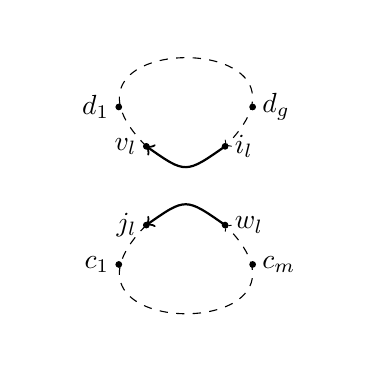
\begin{tikzpicture}[scale=0.50]
\draw[black, thick][<-] (-1,1) .. controls (0,0.3) .. (1,1) ;
\draw[black, thick][<-] (-1,-1) .. controls (0,-0.3) .. (1,-1);
\draw[dashed][->] (-1,-1) .. controls (-4,-4) and (4,-4) ..(1,-1) ;
\draw[dashed][->] (-1,1) .. controls (-4,4) and (4,4) .. (1,1) ;
\filldraw[black] (-1,1) circle (2pt) node[anchor=east]{$v_{l}$};
\filldraw[black] (1,1) circle (2pt) node[anchor=west]{$i_{l}$};
\filldraw[black] (-1,-1) circle (2pt) node[anchor=east]{$j_{l}$};
\filldraw[black] (1,-1) circle (2pt) node[anchor=west]{$w_{l}$};
\filldraw[black] (-1.7,-2) circle (2pt) node[anchor=east]{$c_{1}$};
\filldraw[black] (-1.7,2) circle (2pt) node[anchor=east]{$d_{1}$};
\filldraw[black] (1.7,-2) circle (2pt) node[anchor=west]{$c_{m}$};
\filldraw[black] (1.7,2) circle (2pt) node[anchor=west]{$d_{g}$};
\end{tikzpicture}}; 
\node (positive) [below=of empty] {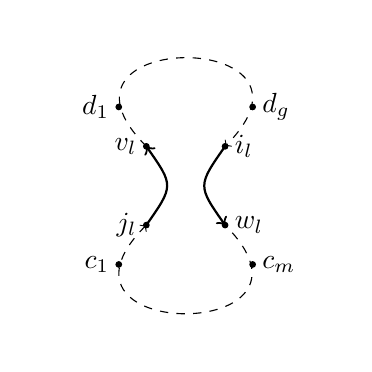
\begin{tikzpicture}[scale=0.50]
\draw[black, thick][->] (-1,-1) .. controls (-0.3,0) .. (-1,1) ;
\draw[black, thick][<-] (1,-1) .. controls (0.3,0) .. (1,1);
\draw[dashed][<-] (-1,-1) .. controls (-4,-4) and (4,-4) ..(1,-1) ;
\draw[dashed][->] (-1,1) .. controls (-4,4) and (4,4) .. (1,1) ;
\filldraw[black] (-1,1) circle (2pt) node[anchor=east]{$v_{l}$};
\filldraw[black] (1,1) circle (2pt) node[anchor=west]{$i_{l}$};
\filldraw[black] (-1,-1) circle (2pt) node[anchor=east]{$j_{l}$};
\filldraw[black] (1,-1) circle (2pt) node[anchor=west]{$w_{l}$};
\filldraw[black] (-1.7,-2) circle (2pt) node[anchor=east]{$c_{1}$};
\filldraw[black] (-1.7,2) circle (2pt) node[anchor=east]{$d_{1}$};
\filldraw[black] (1.7,-2) circle (2pt) node[anchor=west]{$c_{m}$};
\filldraw[black] (1.7,2) circle (2pt) node[anchor=west]{$d_{g}$};
\end{tikzpicture}}; 
\draw[->] (crossing.north) -- (negative.west);
\draw[->] (crossing.south) -- (positive.west);
\end{tikzpicture}
\caption{Case (a): a $1$-smoothing (top) and a $0$-smoothing (bottom) of a positive crossing}
\end{center}
\end{figure}
\item[(b)] \underline{$i_l$ and $v_{l}$ belong to distinct cycles $\cycle{i_{l},j_{l},d_{1},d_{2},\ldots ,d_{g}}$ and $\cycle{w_{l},v_{l},c_{1},c_{2},\ldots ,c_{m}}$ of $\sigma _{\mathbf{v}}^{\omega }$}\\
In this case, a $1$-smoothing of a positive crossing ($\sigma _{\mathbf{v}^{-}}$ if $\epsilon _{l}=1$) or a $0$-smoothing of a negative crossing ($\sigma _{\mathbf{v}^{+}}$ if $\epsilon _{l}=-1$) connects the two cycles into a single cycle $\cycle{i_{l},v_{l},c_{1},\ldots ,c_{m},w_{l},j_{l},d_{1},\ldots ,d_{g}}$. This is done by composing $\sigma _{\mathbf{v}}^{\omega }$ with a single transposition $\cycle{j_{l},v_{l}}$. \\
A $0$-smoothing of a positive crossing ($\sigma _{\mathbf{v}^{+}}$ if $\epsilon _{l}=1$) or a $1$-smoothing of a negative crossing ($\sigma _{\mathbf{v}^{-}}$ if $\epsilon _{l}=-1$) resolves the product of two cycles into a single cycle $\cycle{i_{l},w_{l},c_{m},\ldots ,c_{1},v_{l},j_{l},d_{1},\ldots ,d_{g}}$. Using Lemma \ref{lemma1}, this is achieved by first composing with a transposition $\cycle{j_{l},v_{l}}$ that merges both cycles, and then conjugating with the product of transpositions $\cycle{v_{l},w_{l}}\cycle{c_{1},c_{m}}\ldots \cycle{c_{\lfloor \frac{m}{2}\rfloor},c_{m+1-\lfloor \frac{m}{2}\rfloor }}$. 
\end{itemize} 
\end{proof}

\begin{figure}[H]\label{fig10}
\begin{center}
\begin{tikzpicture}
%\node (crossing) {\begin{tikzpicture}[scale=0.50]
%\draw[black, thick][<-] (-1,-1) -- (1,1);
%\draw[black, thick] (-1,1) -- (-0.1,0.1);
%\draw[black, thick][->] (0.1,-0.1) -- (1,-1);
%\draw[dashed][->] (-1,-1) .. controls (4,-11) and (6,4) ..(1,1) ;
%\draw[dashed][->] (1,-1) .. controls (-4,-11) and (-6,4) .. (-1,1) ;
%\filldraw[black] (-1,1) circle (2pt) node[anchor=south]{$v$};
%\filldraw[black] (1,1) circle (2pt) node[anchor=south]{$i$};
%\filldraw[black] (-1,-1) circle (2pt) node[anchor=north]{$j$};
%\filldraw[black] (1,-1) circle (2pt) node[anchor=north]{$w$};
%\filldraw[black] (-0.5,-3.3) circle (2pt) node[anchor=north]{$c_{1}$};
%\filldraw[black] (-3,1.2) circle (2pt) node[anchor=south]{$c_{m}$};
%\filldraw[black] (0.5,-3.3) circle (2pt) node[anchor=north]{$d_{1}$};
%\filldraw[black] (3,1.2) circle (2pt) node[anchor=south]{$d_{g}$};
%\end{tikzpicture}}; 
\node (negative) {\begin{tikzpicture}[scale=0.50]
\draw[black, thick][<-] (-1,1) .. controls (0,0.3) .. (1,1) ;
\draw[black, thick][<-] (-1,-1) .. controls (0,-0.3) .. (1,-1);
\draw[dashed][->] (-1,-1) .. controls (4,-11) and (6,4) ..(1,1) ;
\draw[dashed][<-] (1,-1) .. controls (-4,-11) and (-6,4) .. (-1,1) ;
\filldraw[black] (-1,1) circle (2pt) node[anchor=south]{$v_{l}$};
\filldraw[black] (1,1) circle (2pt) node[anchor=south]{$i_{l}$};
\filldraw[black] (-1,-1) circle (2pt) node[anchor=east]{$j_{l}$};
\filldraw[black] (1,-1) circle (2pt) node[anchor=west]{$w_{l}$};
\filldraw[black] (-0.5,-3.3) circle (2pt) node[anchor=east]{$c_{1}$};
\filldraw[black] (-3,1.2) circle (2pt) node[anchor=south]{$c_{m}$};
\filldraw[black] (0.5,-3.3) circle (2pt) node[anchor=west]{$d_{1}$};
\filldraw[black] (3,1.2) circle (2pt) node[anchor=south]{$d_{g}$};
\end{tikzpicture}}; 
\node (positive) [right=of negative] {\begin{tikzpicture}[scale=0.50]
\draw[black, thick][<-] (-1,-1) .. controls (-0.3,0) .. (-1,1) ;
\draw[black, thick][<-] (1,-1) .. controls (0.3,0) .. (1,1);
\draw[dashed][->] (-1,-1) .. controls (4,-11) and (6,4) ..(1,1) ;
\draw[dashed][->] (1,-1) .. controls (-4,-11) and (-6,4) .. (-1,1) ;
\filldraw[black] (-1,1) circle (2pt) node[anchor=south]{$v_{l}$};
\filldraw[black] (1,1) circle (2pt) node[anchor=south]{$i_{l}$};
\filldraw[black] (-1,-1) circle (2pt) node[anchor=east]{$j_{l}$};
\filldraw[black] (1,-1) circle (2pt) node[anchor=west]{$w_{l}$};
\filldraw[black] (-0.5,-3.3) circle (2pt) node[anchor=east]{$c_{1}$};
\filldraw[black] (-3,1.2) circle (2pt) node[anchor=south]{$c_{m}$};
\filldraw[black] (0.5,-3.3) circle (2pt) node[anchor=west]{$d_{1}$};
\filldraw[black] (3,1.2) circle (2pt) node[anchor=south]{$d_{g}$};
\end{tikzpicture}}; 
%\draw[->] (crossing.west) -- (negative.east);
%\draw[->] (crossing.east) -- (positive.west);
\end{tikzpicture}
\caption{Case (b): a $1$-smoothing (left) and a $0$-smoothing (right) of a positive crossing}
\end{center}
\end{figure}

\begin{corollary} \label{cor2} Fix an index $l\in \{1,2,\ldots ,k\}$ and let $\mathbf{v}\in \{0,1,2\}^{k}$ be any vector with $\mathbf{v}_{l}=2$. Denote by $\mathbf{v}^{+}$ (resp. $\mathbf{v}^{-}$) the vector obtained from $\mathbf{v}$ by changing $\mathbf{v}_{l}$ to $0$ (resp. 1). Choose an orientation $\omega $ of the smoothing $\Gamma _{\mathbf{v}}$ and denote by $\omega ^{+}$ (resp. $\omega ^{-}$) its induced orientations on the smoothings $\Gamma _{\mathbf{v}^{+}}$ (resp. $\Gamma _{\mathbf{v}^{-}}$). Suppose that $\sigma _{\mathbf{v}}^{\omega }(j_l)=i_{l}$. \begin{enumerate} 
\item Suppose that $\sigma _{\mathbf{v}}^{\omega }(v_l)=w_{l}$. Then we have \begin{enumerate}
\item $(\sigma _{\mathbf{v}^{-\epsilon _{l}}})^{\omega ^{-\epsilon _{l}}}=\sigma _{\mathbf{v}}^{\omega }\cycle{j_{l},v_{l}}$.
\item If $i_l$ and $v_l$ belong to the same cycle $\cycle{j_{l},i_{l},c_{1},c_{2},\ldots ,c_{m},v_{l},w_{l},d_{1}\ldots ,d_{g}}$ of $\sigma _{\mathbf{v}}^{\omega }$, then $$(\sigma _{\mathbf{v}^{\epsilon _{l}}})^{\omega ^{\epsilon _{l}}}=\left (\sigma _{\mathbf{v}}^{\omega }\right )^{\xi _{\mathbf{v}^{\epsilon _{l}},j_{l},w_{l}}}\;.$$
\item If $i_l$ and $v_l$ belong to two distinct cycles $\cycle{j_{l},i_{l},d_{1},d_{2},\ldots ,d_{g}}$ and $\cycle{v_{l},w_{l},c_{1},c_{2},\ldots ,c_{m}}$ of $\sigma _{\mathbf{v}}^{\omega }$, then $$(\sigma _{\mathbf{v}^{\epsilon _{l}}})^{\omega ^{\epsilon _{l}}}=\left (\sigma _{\mathbf{v}}^{\omega }\cycle{j_{l},v_{l}}\right )^{\xi _{\mathbf{v},v_{l},w_{l}}}\;.$$
\end{enumerate}
\item Suppose that $\sigma _{\mathbf{v}}^{\omega }(w_l)=v_{l}$. Then we have
\begin{enumerate}
\item $(\sigma _{\mathbf{v}^{\epsilon _{l}}})^{\omega ^{\epsilon _{l}}}=\sigma _{\mathbf{v}}^{\omega }\cycle{j_{l},w_{l}}$.
\item If $i_l$ and $v_l$ belong to the same cycle $\cycle{j_{l},i_{l},c_{1},c_{2},\ldots ,c_{m},w_{l},v_{l},d_{1}\ldots ,d_{g}}$ of $\sigma _{\mathbf{v}}^{\omega }$, then $$(\sigma _{\mathbf{v}^{-\epsilon _{l}}})^{\omega ^{-\epsilon _{l}}}=\left (\sigma _{\mathbf{v}}^{\omega }\right )^{\xi _{\mathbf{v}^{\epsilon _{l}},j_{l},v_{l}}}\;.$$
\item If $i_l$ and $v_l$ belong to two distinct cycles $\cycle{j_{l},i_{l},d_{1},d_{2},\ldots ,d_{g}}$ and $\cycle{w_{l},v_{l},c_{1},c_{2},\ldots ,c_{m}}$ of $\sigma _{\mathbf{v}}^{\omega }$, then $$(\sigma _{\mathbf{v}^{-\epsilon _{l}}})^{\omega ^{-\epsilon _{l}}}=\left (\sigma _{\mathbf{v}}^{\epsilon _{l}}\cycle{j_{l},w_{l}}\right )^{\xi _{\mathbf{v},v_{l},w_{l}}}\;.$$
\end{enumerate}
\end{enumerate}
\end{corollary}
\begin{proof} In each of the equalities, given by the Theorem \ref{th2}, apply the inverse of the left- and the right-hand side to obtain (1). Do the same with equalities, given by the Theorem \ref{th2}, to obtain (2).  
\end{proof}


\begin{corollary} \label{cor1} Fix an index $l\in \{1,2,\ldots ,k\}$ and let $\mathbf{v}\in \{0,1,2\}^{k}$ be any vector with $\mathbf{v}_{l}=2$. Denote by $\mathbf{v}^{+}$ (resp. $\mathbf{v}^{-}$) the vector obtained from $\mathbf{v}$ by changing $\mathbf{v}_{l}$ to $0$ (resp. 1). Choose an orientation $\omega $ of the smoothing $\Gamma _{\mathbf{v}}$ and denote by $\omega ^{+}$ (resp. $\omega ^{-}$) its induced orientations on the smoothings $\Gamma _{\mathbf{v}^{+}}$ (resp. $\Gamma _{\mathbf{v}^{-}}$). Let $\{a,b\}=\{v_{l},w_{l}\}$. Then we have \begin{enumerate}
\item If $i_l$ and $v_l$ belong to distinct cycles of $\sigma _{\mathbf{v}}^{\omega }$, then $(\sigma _{\mathbf{v}^{-}})^{\omega ^{-}}=\left (\sigma _{\mathbf{v}^{+}}^{\omega ^{+}}\right )^{\xi _{\mathbf{v},v_{l},w_{l}}}$. 
\item Suppose that $i_l$ and $v_l$ belong to the same cycle of $\sigma _{\mathbf{v}}^{\omega }$ and $\sigma _{\mathbf{v}}^{\omega }(a)=b$.\\ If $\sigma _{\mathbf{v}}^{\omega }(i_l)=j_{l}$, then $$(\sigma _{\mathbf{v}^{-}})^{\omega ^{-}}=\begin{cases} \cycle{j_{l},b}\left (\sigma _{\mathbf{v}^{+}}^{\omega ^{+}}\right )^{\xi _{\mathbf{v}^{-},j_{l},a}}\;, & (a=w_{l}\land \epsilon _{l}=1)\lor (a=v_{l}\land \epsilon _{l}=-1)\\
\left (\cycle{j_{l},b}\sigma _{\mathbf{v}^{+}}^{\omega ^{+}}\right )^{\xi _{\mathbf{v}^{+},j_{l},a}}\;, & (a=w_{l}\land \epsilon _{l}=-1)\lor (a=v_{l}\land \epsilon _{l}=1)\;.
\end{cases}$$
If $\sigma _{\mathbf{v}}^{\omega }(j_l)=i_{l}$, then $$(\sigma _{\mathbf{v}^{-}})^{\omega ^{-}}=\begin{cases} \left (\sigma _{\mathbf{v}^{+}}^{\omega ^{+}}\cycle{j_{l},a}\right )^{\xi _{\mathbf{v}^{+},j_{l},b}}\;, & (a=v_{l}\land \epsilon _{l}=-1)\lor (a=w_{l}\land \epsilon _{l}=1)\\
\left (\sigma _{\mathbf{v}^{+}}^{\omega ^{+}} \right )^{\xi _{\mathbf{v}^{-},j_{l},b}}\cycle{j_{l},a}\;, & (a=v_{l}\land \epsilon _{l}=1)\lor (a=w_{l}\land \epsilon _{l}=-1)\;.
\end{cases}$$
\end{enumerate}
\end{corollary}
\begin{proof} The claimed relationship between the two resolutions follows from Theorem \ref{th1}, Theorem \ref{th2} and Corollary \ref{cor2} by a straightforward computation. 
\end{proof}


To every smoothing $\Gamma _{\mathbf{v}}$ in the cube of smoothings, we have associated a group $G_{\mathbf{v}}$ that is a direct product of dihedral groups, corresponding to the components of $\Gamma _{\mathbf{v}}$. Now we consider the cobordism $W_{\zeta }$, corresponding to an edge $\mathbf{v}\stackrel{\zeta}{\rightarrow}\mathbf{v}'$, and describe the relationship between its vertex groups $G_{\mathbf{v}}$, $G_{\mathbf{v}'}$. Any cylindrical component of $W_{\zeta }$, bounded by two identical circles in $\Gamma _{\mathbf{v}}$ and $\Gamma _{\mathbf{v}'}$, gives rise to the identity between the corresponding factors of $G_{\mathbf{v}}$ resp. $G_{\mathbf{v}'}$. The nontrivial relationship occurs in the factors associated with the ``pair of pants'' cobordism. \\

Let us denote by $G_{\mathbf{v},a}$ the factor of $G_{\mathbf{v}}$ that corresponds to the component of $\Gamma _{\mathbf{v}}$ containing the vertex $q_{a}$. 

\begin{proposition} \label{prop1} Let $\mathbf{v}''\in \{0,1,2\}^{k}$ be any vector with $\mathbf{v}''_{l}=2$ for some index $l\in \{1,2,\ldots ,k\}$. Suppose that two smoothings $\Gamma _{\mathbf{v}}$ and $\Gamma _{\mathbf{v}'}$ are obtained as the $0$- and $1$-smoothing of the $l$-th crossing $\overline{q_{i_{l}}q_{j_{l}}}\cap \overline{q_{v_{l}}q_{w_{l}}}$ respectively, so that the edge $\mathbf{v}\stackrel{\zeta}{\rightarrow}\mathbf{v}'$ is given by a $\star $ at the $l$-th position. Let $\omega ''$ be an orientation of the partial smoothing $\Gamma _{\mathbf{v''}}$, for which $\sigma _{\mathbf{v}''}^{\omega ''}(i_{l})=j_l$ and $\sigma _{\mathbf{v}''}^{\omega ''}(a)=b$, where $\{a,b\}=\{v,w\}$. Let $\omega $ (resp. $\omega '$) be the orientations for $\Gamma _{\mathbf{v}}$ (resp. $\Gamma _{\mathbf{v}'}$) that are both induced from $\omega ''$ on $\Gamma _{\mathbf{v''}}$. Then the following holds. \begin{enumerate}
\item If the vertices $q_{i_{l}}$ and $q_{j_{l}}$ belong to two distinct components of the smoothing $\Gamma _{\mathbf{v}}$, then the generators of the vertex groups $G_{\mathbf{v},i_{l}}\times G_{\mathbf{v},j_{l}}$ and $G_{\mathbf{v}',i_{l}}$ are related by
\begin{xalignat*}{1}
& \lambda _{\mathbf{v}',i_{l},j_{l}}^{\omega'}=\left (\cycle{j_{l},b}\lambda _{\mathbf{v},j_{l},a}^{\omega}\,\lambda _{\mathbf{v},i_{l},b}^{\omega}\right )^{\xi _{\mathbf{v},j_{l},a}}\quad \textrm{if ($\epsilon _{l}=1\land a=v_{l}$) or ($\epsilon _{l}=-1\land a=w_{l}$)}\;.\\
& \xi _{\mathbf{v}',i_{l},w_{l}}=\xi _{\mathbf{v},i_{l},w_{l}}\xi _{\mathbf{v},j_{l},v_{l}}\;,  \textrm{ if }\epsilon _{l}=1\;,\\
& \xi _{\mathbf{v}',i_{l},v_{l}}=\xi _{\mathbf{v},i_{l},v_{l}}\xi _{\mathbf{v},j_{l},w_{l}}\;,  \textrm{ if }\epsilon _{l}=-1\;. 
\end{xalignat*}
\item If the vertices $q_{i_{l}}$ and $q_{j_{l}}$ belong to the same component of the smoothing $\Gamma _{\mathbf{v}}$, then the generators of the vertex groups $G_{\mathbf{v},i_{l}}$ and $G_{\mathbf{v}',i_{l}}\times G_{\mathbf{v}',j_{l}}$ are related by
\begin{xalignat*}{1}
& \lambda _{\mathbf{v}',i_{l},b}^{\omega'}\,\lambda _{\mathbf{v}',j_{l},a}^{\omega'}=\cycle{j_{l},b}\left (\lambda _{\mathbf{v},i_{l},j_{l}}^{\omega }\right )^{\xi _{\mathbf{v}',j_{l},a}}\;, \quad \textrm{if ($\epsilon _{l}=1\land a=w_{l}$) or ($\epsilon _{l}=-1\land a=v_{l}$)}\;.\\
& \xi _{\mathbf{v}',i_{l},v_{l}}\xi _{\mathbf{v}',j_{l},w_{l}}= \xi _{\mathbf{v},i_{l},v_{l}}\;,  \textrm{ if }\epsilon _{l}=1\;,\\
& \xi _{\mathbf{v}',i_{l},w_{l}}\xi _{\mathbf{v}',j_{l},v_{l}}= \xi _{\mathbf{v},i_{l},w_{l}}\;,  \textrm{ if }\epsilon _{l}=-1\;,
\end{xalignat*}
\end{enumerate}
\end{proposition}

\begin{proof} We apply a case analysis in Corollary \ref{cor1} (2). \end{proof}
\begin{figure}[H]\label{fig11}
\begin{center}
\begin{tikzpicture}
\node (zero)   {\begin{tikzpicture}[scale=0.50]
\draw[black, thick][<-] (-1,-1) .. controls (-0.3,0) .. (-1,1) ;
\draw[black, thick][<-] (1,-1) .. controls (0.3,0) .. (1,1);
\draw[dashed][->] (-1,-1) .. controls (-6,-4) and (-6,4) ..(-1,1) ;
\draw[dashed][<-] (1,1) .. controls (6,4) and (6,-4) .. (1,-1) ;
\filldraw[black] (-1,1) circle (2pt) node[anchor=south]{$v_l$};
\filldraw[black] (1,1) circle (2pt) node[anchor=south]{$i_l$};
\filldraw[black] (-1,-1) circle (2pt) node[anchor=north]{$j_l$};
\filldraw[black] (1,-1) circle (2pt) node[anchor=north]{$w_l$};
\filldraw[black] (-3,-1.75) circle (2pt) node[anchor=north]{$c_{1}$};
\filldraw[black] (-3,1.75) circle (2pt) node[anchor=south]{$c_{m}$};
\filldraw[black] (3,-1.75) circle (2pt) node[anchor=north]{$d_{1}$};
\filldraw[black] (3,1.75) circle (2pt) node[anchor=south]{$d_{g}$};
\end{tikzpicture}}; 
\node (one) [right=of zero] {\begin{tikzpicture}[scale=0.50]
\draw[black, thick][<-] (-1,1) .. controls (0,0.3) .. (1,1) ;
\draw[black, thick][->] (-1,-1) .. controls (0,-0.3) .. (1,-1);
\draw[dashed][->] (-1,-1) .. controls (-6,-4) and (-6,4) ..(-1,1) ;
\draw[dashed][<-] (1,1) .. controls (6,4) and (6,-4) .. (1,-1) ;
\filldraw[black] (-1,1) circle (2pt) node[anchor=south]{$v_l$};
\filldraw[black] (1,1) circle (2pt) node[anchor=south]{$i_l$};
\filldraw[black] (-1,-1) circle (2pt) node[anchor=north]{$j_l$};
\filldraw[black] (1,-1) circle (2pt) node[anchor=north]{$w_l$};
\filldraw[black] (-3,-1.75) circle (2pt) node[anchor=north]{$c_{1}$};
\filldraw[black] (-3,1.75) circle (2pt) node[anchor=south]{$c_{m}$};
\filldraw[black] (3,-1.75) circle (2pt) node[anchor=north]{$d_{1}$};
\filldraw[black] (3,1.75) circle (2pt) node[anchor=south]{$d_{g}$};
\end{tikzpicture}}; 
\draw[red] (zero.west) -- (zero.east);
\draw[red] (one.west) -- (one.east);
\end{tikzpicture}
\caption{Reflection of a cobordism: a $0$-smoothing (left) and a $1$-smoothing (right) of a positive crossing}
\end{center}
\end{figure}


A polygonal link representation endows the cube of smoothings with a combinatorial structure, given by the cube of groups $G_{\mathbf{v}}$ and relationships between their generators, described in the Proposition \ref{prop1}. These relationships are based on \begin{itemize}
\item multiplication by a transposition of two indices of the vertices in a crossing,
\item conjugation by the order 2 elements of the vertex groups.  
\end{itemize} 
To study possible link invariants, based on this structure, we need to describe the moves between equivalent structures, i.e., what happens to the cube of groups during a deformation of a link component. Recall that an elementary deformation consists of changing a good link diagram $\left ((q_{1},\ldots ,q_{n_{1}}),(q_{n_{1}+1},\ldots ,q_{n_{2}}),\ldots (q_{n_{r-1}+1},\ldots ,q_{n_r})\right )$ by \begin{itemize}
\item[(I)] adding a new vertex $q_{n+1}$ to a link component, and replacing an edge $\overline{q_{l}q_{m}}$ by new edges $\overline{q_{l}q_{n+1}}$ and $\overline{q_{n+1}q_{m}}$, or
\item[(II)] removing a vertex $q_{p}$ from a link component and replacing both edges $\overline{q_{l}q_{p}}$ and $\overline{q_{p}q_{m}}$, incident at this vertex, by a new edge $\overline{q_{l}q_{m}}$.
\end{itemize}
It is sufficient to know what happens under a deformation of type (II). We assume that both the original and the deformed diagram are good diagrams, thus each of the sides $\overline{q_{l}q_{p}}$, $\overline{q_{m}q_{p}}$ and $\overline{q_{l}q_{m}}$ contains at most one crossing. Every other edge of our diagram may intersect either $0$, $1$ or $2$ edges of the triangle $T$.
Let us denote by $\widehat{G}_{\mathbf{v}}$ (resp. $\widehat{\lambda} _{\mathbf{v},l}$) the group of the deformed diagram (resp. its generator, corresponding to the component containing the vertex $q_{l}$). \\

First assume that in our diagram, the triangle $T=\overline{q_{l}q_{m}q_{p}}$ contains no other vertex projections than $q_{l}$, $q_{m}$ and $q_{p}$. In this case, we have 5 possible situations (see Figure \ref{fig12}):
\begin{enumerate}
\item No edge of the triangle $T$ contains any crossings. It follows that $G_{\mathbf{v},l}=G_{\mathbf{v},m}=G_{\mathbf{v},p}$ and $$\widehat{\lambda }_{\mathbf{v},l}=\begin{cases} \lambda _{\mathbf{v},l}\cycle{l,p}\quad \textrm{ if $\lambda _{\mathbf{v},l}(l)=m$}\\
\lambda _{\mathbf{v},l}\cycle{m,p}\quad \textrm{ if $\lambda _{\mathbf{v},l}(m)=l$}\end{cases}$$ for every smoothing vector $\mathbf{v}\in \{0,1\}^{k}$. 
\item The edge $\overline{q_{l}q_{p}}$ has one crossing with an edge $\overline{q_{m}q_{a}}$, while the remaining two sides of $T$ contain no crossings. Under the deformation, the crossing disappears. \\
This situation describes a polygonal Reidemeister I move. The two smoothings of the initial cycle $\lambda _{2^{k},l}=\cycle{l,p,m,a,c_{1},\ldots ,c_{b}}$ are given as $\cycle{l,a,c_{1},\ldots ,c_{b}}\cycle{p,m}=\cycle{a,p}\lambda _{2^{k},l}$ and $\cycle{l,m,p,a,c_{1},\ldots ,c_{b}}=\lambda _{2^{k},l}^{\cycle{m,p}}$. The deformed cycle equals $\widehat{\lambda}_{\mathbf{v},l}=\cycle{l,m,a,c_{1},\ldots ,c_{b}}=\lambda _{2^{k},l}\cycle{l,p}$. Thus we obtain $$\widehat{\lambda }_{\mathbf{v},l}=\begin{cases}
\cycle{a,p}\lambda _{\mathbf{v},l}\cycle{l,p} & \textrm{if }\lambda _{\mathbf{v},l}\neq \lambda_{\mathbf{v},m}\\
\left (\lambda _{\mathbf{v},l}\right )^{\cycle{m,p}}\cycle{l,p} & \textrm{if }\lambda _{\mathbf{v},l}=\lambda_{\mathbf{v},m}
\end{cases}$$ In the case when $\lambda _{\mathbf{v},l}\neq \lambda_{\mathbf{v},m}$, we have $G_{\mathbf{v},m}\cong \ZZ _{2}\langle \cycle{p,m}\rangle $.
\item The edge $\overline{q_{m}q_{p}}$ has one crossing with another edge $\overline{q_{l}q_{a}}$, while the remaining two sides of $T$ contain no crossings. Under the deformation, the crossing disappears. Here we just reverse the roles of the indices $l$ and $m$ in the case (2) and obtain 
$$\widehat{\lambda }_{\mathbf{v},m}=\begin{cases}
\cycle{a,p}\lambda _{\mathbf{v},m}\cycle{m,p} & \textrm{if }\lambda _{\mathbf{v},m}\neq \lambda_{\mathbf{v},l}\\
\left (\lambda _{\mathbf{v},m}\right )^{\cycle{l,p}}\cycle{m,p} & \textrm{if }\lambda _{\mathbf{v},m}=\lambda_{\mathbf{v},l}
\end{cases}$$ In the case when $\lambda _{\mathbf{v},m}\neq \lambda_{\mathbf{v},l}$, we have $G_{\mathbf{v},l}\cong \ZZ _{2}\langle \cycle{p,l}\rangle $.
\item The initial edge $\overline{q_{l}q_{p}}$ and the deformed edge $\overline{q_{l}q_{m}}$ both have one crossing with an edge $\overline{q_{a}q_{b}}$, while the third edge of the triangle $T$ contains no crossings. \\
Any two smoothings of the initial diagram that differ only at the crossing $\overline{q_{l}q_{p}}\cap \overline{q_{a}q_{b}}$, are given by permutations $\sigma _{0}$ and $\sigma _{1}$, for which we have $\sigma _{0}^{\pm 1}(p)=m$ and $\sigma _{1}^{\pm 1}(p)=m$ (the plus or minus sign depends on the orientation of a smoothing). The permutations of the transformed smoothings are then obtained by left or right multiplication with the transposition $\cycle{m,p}$. Moreover, this deformation changes the quadruple of crossing indices $i,j,v,w$ (the index $p$ is exchanged for the index $m$). 
\item The initial edge $\overline{q_{p}q_{m}}$ and the deformed edge $\overline{q_{l}q_{m}}$ both have one crossing with an edge $\overline{q_{a}q_{b}}$, while the third edge of the triangle $T$ contains no crossings. Analogous reasoning as in the case (4) implies that permutations of the deformed smoothings are obtained by either left or right multiplication with the transposition $\cycle{l,p}$. The quadruple of crossing indices $i,j,v,w$ is transformed (the index $p$ is exchanged for the index $l$). 
\end{enumerate}
\begin{figure}[H]
\begin{tikzpicture}
\matrix [column sep=1cm]
{
\node {\begin{tikzpicture}
\draw[dashed] (-1,-1) -- (1,-1);
\draw[black, thick] (-1,-1) -- (0,0);
\draw[black, thick] (1,-1) -- (0,0);
\filldraw[black] (-1,-1) circle (2pt) node[anchor=east]{$l$};
\filldraw[black] (1,-1) circle (2pt) node[anchor=west]{$m$};
\filldraw[black] (0,0) circle (2pt) node[anchor=east]{$p$};
\end{tikzpicture}}; & \node {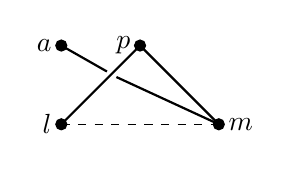
\begin{tikzpicture}
\draw[dashed] (-1,-1) -- (1,-1);
\draw[black, thick] (-1,-1) -- (0,0);
\draw[black, thick] (1,-1) -- (0,0);
\draw[black, thick] (1,-1) -- (-0.3,-0.4);
\draw[black, thick] (-0.42,-0.33) -- (-1,0);
\filldraw[black] (-1,-1) circle (2pt) node[anchor=east]{$l$};
\filldraw[black] (1,-1) circle (2pt) node[anchor=west]{$m$};
\filldraw[black] (0,0) circle (2pt) node[anchor=east]{$p$};
\filldraw[black] (-1,0) circle (2pt) node[anchor=east]{$a$};
\end{tikzpicture}}; & \node {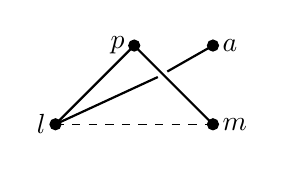
\begin{tikzpicture}
\draw[dashed] (-1,-1) -- (1,-1);
\draw[black, thick] (-1,-1) -- (0,0);
\draw[black, thick] (1,-1) -- (0,0);
\draw[black, thick] (-1,-1) -- (0.3,-0.4);
\draw[black, thick] (0.42,-0.33) -- (1,0);
\filldraw[black] (-1,-1) circle (2pt) node[anchor=east]{$l$};
\filldraw[black] (1,-1) circle (2pt) node[anchor=west]{$m$};
\filldraw[black] (0,0) circle (2pt) node[anchor=east]{$p$};
\filldraw[black] (1,0) circle (2pt) node[anchor=west]{$a$};
\end{tikzpicture}};\\
\node {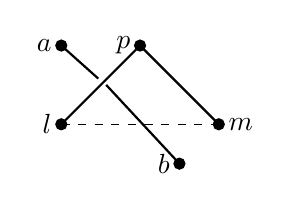
\begin{tikzpicture}
\draw[dashed] (-1,-1) -- (1,-1);
\draw[black, thick] (-1,-1) -- (0,0);
\draw[black, thick] (1,-1) -- (0,0);
\draw[black, thick] (0.5,-1.5) -- (-0.43,-0.5);
\draw[black, thick] (-0.53,-0.42) -- (-1,0);
\filldraw[black] (-1,-1) circle (2pt) node[anchor=east]{$l$};
\filldraw[black] (1,-1) circle (2pt) node[anchor=west]{$m$};
\filldraw[black] (0,0) circle (2pt) node[anchor=east]{$p$};
\filldraw[black] (-1,0) circle (2pt) node[anchor=east]{$a$};
\filldraw[black] (0.5,-1.5) circle (2pt) node[anchor=east]{$b$};
\end{tikzpicture}}; & \node {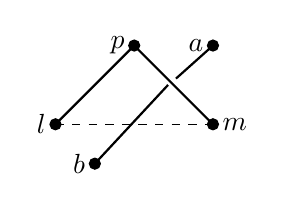
\begin{tikzpicture}
\draw[dashed] (-1,-1) -- (1,-1);
\draw[black, thick] (-1,-1) -- (0,0);
\draw[black, thick] (1,-1) -- (0,0);
\draw[black, thick] (-0.5,-1.5) -- (0.43,-0.5);
\draw[black, thick] (0.53,-0.42) -- (1,0);
\filldraw[black] (-1,-1) circle (2pt) node[anchor=east]{$l$};
\filldraw[black] (1,-1) circle (2pt) node[anchor=west]{$m$};
\filldraw[black] (0,0) circle (2pt) node[anchor=east]{$p$};
\filldraw[black] (1,0) circle (2pt) node[anchor=east]{$a$};
\filldraw[black] (-0.5,-1.5) circle (2pt) node[anchor=east]{$b$};
\end{tikzpicture}}; & \node {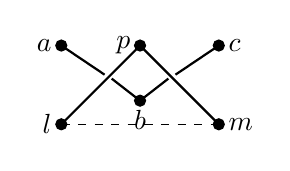
\begin{tikzpicture}
\draw[dashed] (-1,-1) -- (1,-1);
\draw[black, thick] (-1,-1) -- (0,0);
\draw[black, thick] (1,-1) -- (0,0);
\draw[black, thick] (0,-0.7) -- (0.36,-0.42);
\draw[black, thick] (0.45,-0.37) -- (1,0);
\draw[black, thick] (0,-0.7) -- (-0.36,-0.42);
\draw[black, thick](-0.45,-0.37) -- (-1,0);
\filldraw[black] (-1,-1) circle (2pt) node[anchor=east]{$l$};
\filldraw[black] (1,-1) circle (2pt) node[anchor=west]{$m$};
\filldraw[black] (0,0) circle (2pt) node[anchor=east]{$p$};
\filldraw[black] (1,0) circle (2pt) node[anchor=west]{$c$};
\filldraw[black] (0,-0.7) circle (2pt) node[anchor=north]{$b$};
\filldraw[black] (-1,0) circle (2pt) node[anchor=east]{$a$};
\end{tikzpicture}}; \\
};
\end{tikzpicture}
\caption{Local deformations of a good diagram. The top pictures show the cases (1),(2),(3), and the bottom pictures show the cases (4),(5),(c). }
\label{fig12}
\end{figure}

Our analysis of polygonal deformations implies the following result. 

\begin{proposition} Let us have a cube of smoothings of a good link diagram $\mathcal{D}$ with $n$ vertices $q_{1},q_{2},\ldots ,q_{n}$ and $k$ crossings.\begin{enumerate}
\item Suppose that every smoothing $\Gamma _{\mathbf{v}}$ admits an orientation $\omega _{\mathbf{v}}$, for which the permutation $\sigma _{\mathbf{v}}^{\omega _{\mathbf{v}}}$ has $\sigma _{\mathbf{v}}^{\omega _{\mathbf{v}}}(l)=p$ and $\sigma _{\mathbf{v}}^{\omega _{\mathbf{v}}}(p)=m$. Then the cube of permutations $\{\sigma _{\mathbf{v}}^{\omega _{\mathbf{v}}}\colon \mathbf{v}\in \{0,1\}^{k}\}$ is equivalent to a deformed cube of permutations $\{\sigma _{\mathbf{v}}^{\omega _{\mathbf{v}}}\cycle{l,p}\colon \mathbf{v}\in \{0,1\}^{k}\}$.
\item Suppose that there exists an index $l\in \{1,2,\ldots ,k\}$ and some $\rho \in \{0,1\}$, such that $G_{\mathbf{v}}=\ZZ _{2}\langle \cycle{m,p}\rangle $ for every $\mathbf{v}\in \{0,1\}^{k}$ with $\mathbf{v}_{l}=\rho$, while every smoothing $\Gamma _{\mathbf{v}}$ for $\mathbf{v}_{l}\neq \rho$ admits an orientation $\omega _{\mathbf{v}}$, for which $\sigma _{\mathbf{v}}^{\omega _{\mathbf{v}}}(l)=m$ and $\sigma _{\mathbf{v}}^{\omega _{\mathbf{v}}}(m)=p$. Then the cube of permutations $\{\sigma _{\mathbf{v}}^{\omega _{\mathbf{v}}}\colon \mathbf{v}\in \{0,1\}^{k}\}$ is equivalent to a deformed cube of permutations $\{\sigma _{\mathbf{v}}^{\omega _{\mathbf{v}}}\cycle{m,p}\colon \mathbf{v}\in \{0,1\}^{k}\land \mathbf{v}_{l}=\rho \}$.
\end{enumerate}
\end{proposition}

Now suppose that the triangle $T$ contains one other vertex projection $q_{a}$ appart from $q_{l}$, $q_{m}$ and $q_{p}$. We have 3 basic possibilities:
\begin{enumerate}
\item [(a)] One of the edges $\overline{q_{l}q_{p}}$, $\overline{q_{p}q_{m}}$ has a crossing with an edge $\overline{q_{a}q_{b}}$, while the remaining two sides of $T$ contain no crossings. It follows that the vertex $q_{a}$ must be adjacent to one of the vertices $q_{l}$, $q_{m}$. Then our transformation is either a composition of a transformation of type (2) or (3) and a transformation of type (1), or a composition of two type (1) transformations. 
\item [(b)] One of the initial edges $\overline{q_{l}q_{p}}$ and $\overline{q_{p}q_{m}}$ has a crossing with an edge $\overline{q_{a}q_{b}}$, while the deformed edge $\overline{q_{l}q_{m}}$ has a crossing with an edge $\overline{q_{a}q_{c}}$. Then our transformation is a composition of a transformation of type (4) or (5) and a transformation of type (1).
\item [(c)]The initial edge $\overline{q_{l}q_{p}}$ has a crossing with an edge $\overline{q_{a}q_{b}}$ and the initial edge $\overline{q_{p}q_{m}}$ has a crossing with an edge $\overline{q_{a}q_{c}}$, while the deformed edge contains no crossings. This is a new situation, describing a polygonal Reidemeister II move. In this case two crossings that share two crossing vertices disappear. The two crossings in the initial diagram give rise to four distinct smoothings of the local picture (see Figure \ref{fig13}); one of them contains a bigon whose group is of order 2. 
%We may compute
%\begin{xalignat*}{1}
%& \cycle{a,p}\cycle{a,b}\cycle{a,m}\cycle{l,a,\ldots}\cycle{b,p}\cycle{c,m,\ldots }=\cycle{l,m,\ldots }\cycle{c,b,a,\ldots }\\
%& \cycle{b,p}\cycle{a,m}\cycle{l,a,\ldots}\cycle{c,p,b,m,\ldots }=\cycle{l,m,\ldots }\cycle{c,b,a,\ldots }\\
%& \cycle{a,p}\cycle{b,m}\cycle{l,b,p,a,\ldots}\cycle{c,m,\ldots }=\cycle{l,m,\ldots }\cycle{c,b,a,\ldots }\\
%& \cycle{b,p}\cycle{b,m}\cycle{a,p,c,\ldots}\cycle{l,b,m,\ldots }\cycle{b,p}=\cycle{l,m,\ldots }\cycle{a,b,c,\ldots }
%\end{xalignat*}
\end{enumerate}

\begin{figure}[H]
\begin{tikzpicture}
\matrix [column sep=0.7cm]
{
& \node {\begin{tikzpicture}
\draw[dashed] (-1,-1) -- (-1.7,-1.2);
\draw[dashed] (1,-1) -- (1.7,-1.2);
\draw[dashed] (-1,0) -- (-1.7,0.2);
\draw[dashed] (1,0) -- (1.7,0.2);
\draw[black, thick] (-1,-1) -- (0,0);
\draw[black, thick] (1,-1) -- (0,0);
\draw[black, thick] (0,-0.7) -- (0.36,-0.42);
\draw[black, thick] (0.45,-0.37) -- (1,0);
\draw[black, thick] (0,-0.7) -- (-0.36,-0.42);
\draw[black, thick](-0.45,-0.37) -- (-1,0);
\filldraw[black] (-1,-1) circle (2pt) node[anchor=north]{$l$};
\filldraw[black] (1,-1) circle (2pt) node[anchor=north]{$m$};
\filldraw[black] (0,0) circle (2pt) node[anchor=south]{$p$};
\filldraw[black] (1,0) circle (2pt) node[anchor=south]{$c$};
\filldraw[black] (0,-0.7) circle (2pt) node[anchor=north]{$b$};
\filldraw[black] (-1,0) circle (2pt) node[anchor=south]{$a$};
\end{tikzpicture}}; 
& \node {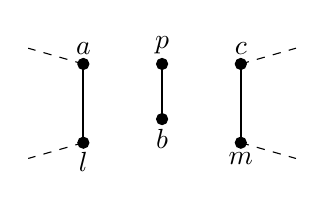
\begin{tikzpicture}
\draw[dashed] (-1,-1) -- (-1.7,-1.2);
\draw[dashed] (1,-1) -- (1.7,-1.2);
\draw[dashed] (-1,0) -- (-1.7,0.2);
\draw[dashed] (1,0) -- (1.7,0.2);
\draw[black, thick] (-1,-1) -- (-1,0);
\draw[black, thick] (1,-1) -- (1,0);
\draw[black, thick] (0,-0.7) -- (0,0);
\filldraw[black] (-1,-1) circle (2pt) node[anchor=north]{$l$};
\filldraw[black] (1,-1) circle (2pt) node[anchor=north]{$m$};
\filldraw[black] (0,0) circle (2pt) node[anchor=south]{$p$};
\filldraw[black] (1,0) circle (2pt) node[anchor=south]{$c$};
\filldraw[black] (0,-0.7) circle (2pt) node[anchor=north]{$b$};
\filldraw[black] (-1,0) circle (2pt) node[anchor=south]{$a$};
\end{tikzpicture}};
& \node {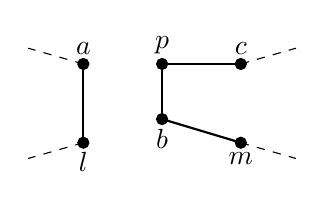
\begin{tikzpicture}
\draw[dashed] (-1,-1) -- (-1.7,-1.2);
\draw[dashed] (1,-1) -- (1.7,-1.2);
\draw[dashed] (-1,0) -- (-1.7,0.2);
\draw[dashed] (1,0) -- (1.7,0.2);
\draw[black, thick] (-1,-1) -- (-1,0);
\draw[black, thick] (1,-1) -- (0,-0.7);
\draw[black, thick] (1,0) -- (0,0);
\draw[black, thick] (0,-0.7) -- (0,0);
\filldraw[black] (-1,-1) circle (2pt) node[anchor=north]{$l$};
\filldraw[black] (1,-1) circle (2pt) node[anchor=north]{$m$};
\filldraw[black] (0,0) circle (2pt) node[anchor=south]{$p$};
\filldraw[black] (1,0) circle (2pt) node[anchor=south]{$c$};
\filldraw[black] (0,-0.7) circle (2pt) node[anchor=north]{$b$};
\filldraw[black] (-1,0) circle (2pt) node[anchor=south]{$a$};
\end{tikzpicture}};\\
& \node {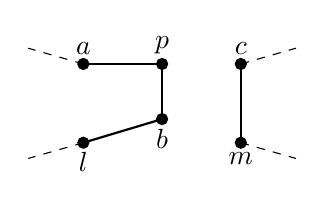
\begin{tikzpicture}
\draw[dashed] (-1,-1) -- (-1.7,-1.2);
\draw[dashed] (1,-1) -- (1.7,-1.2);
\draw[dashed] (-1,0) -- (-1.7,0.2);
\draw[dashed] (1,0) -- (1.7,0.2);
\draw[black, thick] (-1,-1) -- (0,-0.7);
\draw[black, thick] (-1,0) -- (0,0);
\draw[black, thick] (0,-0.7) -- (0,0);
\draw[black, thick] (1,-1) -- (1,0);
\filldraw[black] (-1,-1) circle (2pt) node[anchor=north]{$l$};
\filldraw[black] (1,-1) circle (2pt) node[anchor=north]{$m$};
\filldraw[black] (0,0) circle (2pt) node[anchor=south]{$p$};
\filldraw[black] (1,0) circle (2pt) node[anchor=south]{$c$};
\filldraw[black] (0,-0.7) circle (2pt) node[anchor=north]{$b$};
\filldraw[black] (-1,0) circle (2pt) node[anchor=south]{$a$};
\end{tikzpicture}};
& \node {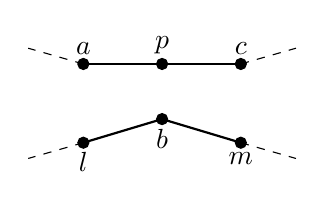
\begin{tikzpicture}
\draw[dashed] (-1,-1) -- (-1.7,-1.2);
\draw[dashed] (1,-1) -- (1.7,-1.2);
\draw[dashed] (-1,0) -- (-1.7,0.2);
\draw[dashed] (1,0) -- (1.7,0.2);
\draw[black, thick] (-1,-1) -- (0,-0.7);
\draw[black, thick] (0,-0.7) -- (1,-1);
\draw[black, thick] (-1,0) -- (0,0);
\draw[black, thick] (0,0) -- (1,0);
\filldraw[black] (-1,-1) circle (2pt) node[anchor=north]{$l$};
\filldraw[black] (1,-1) circle (2pt) node[anchor=north]{$m$};
\filldraw[black] (0,0) circle (2pt) node[anchor=south]{$p$};
\filldraw[black] (1,0) circle (2pt) node[anchor=south]{$c$};
\filldraw[black] (0,-0.7) circle (2pt) node[anchor=north]{$b$};
\filldraw[black] (-1,0) circle (2pt) node[anchor=south]{$a$};
\end{tikzpicture}};
& \node {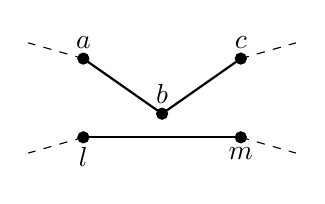
\begin{tikzpicture}
\draw[dashed] (-1,-1) -- (-1.7,-1.2);
\draw[dashed] (1,-1) -- (1.7,-1.2);
\draw[dashed] (-1,0) -- (-1.7,0.2);
\draw[dashed] (1,0) -- (1.7,0.2);
\draw[black, thick] (-1,-1) -- (1,-1);
\draw[black, thick] (0,-0.7) -- (1,0);
\draw[black, thick] (0,-0.7) -- (-1,0);
\filldraw[black] (-1,-1) circle (2pt) node[anchor=north]{$l$};
\filldraw[black] (1,-1) circle (2pt) node[anchor=north]{$m$};
\filldraw[black] (1,0) circle (2pt) node[anchor=south]{$c$};
\filldraw[black] (0,-0.7) circle (2pt) node[anchor=south]{$b$};
\filldraw[black] (-1,0) circle (2pt) node[anchor=south]{$a$};
\end{tikzpicture}};\\
};
\end{tikzpicture}
\caption{Case (c): the initial diagram (top left) with its four smoothings and the deformed diagram (bottom right). }
\label{fig13}
\end{figure}

The polygonal Reidemeister III move of a good diagram is depicted in Figure \ref{fig14}. It appears as a composition of type (1) moves (the intermediate steps in this composition are not good diagrams). This transformation changes a triple of crossings, such that any two crossings in the triple share a common crossing vertex, into another triple of crossings with the same property. A curious transformation in the crossing role of nine vertices happens. Choosing one possible orientation, we have labelled the vertices in accordance with the initial triple of crossings by $i_{l},j_{l},v_{l},w_{l}$ for $l=1,2,3$. The (capital) vertex labellings of the transformed crossings correspond as follows: $(I_{1}=i_{1},J_{1}=j_{1}', V_{1}=v_{3}', W_{1}=w_{3}), (I_{2}=i_{2}', J_{2}=j_{2}, V_{2}=i_{3}, W_{2}=j_{3}'), (I_{3}=v_{1}', J_{3}=w_{1}, V_{3}=v_{2},W_{3}=w_{2}')$.  

\begin{figure}[H]
\begin{tikzpicture}
\matrix [column sep=0.7cm]
{
& \node {\begin{tikzpicture}
\draw[dashed] (-1,-1) -- (-1.7,-1.2);
\draw[dashed] (-1,0) -- (-1.7,0);
\draw[dashed] (-1,1) -- (-1.7,1.2);
\draw[dashed] (1,0) -- (1.7,0);
\draw[dashed] (1,1) -- (1.7,1.2);
\draw[dashed] (1,-1) -- (1.7,-1.2);
\draw[black, thick] (-1,1) -- (-0.5,-0.5);
\draw[black, thick] (-1,0) -- (-0.78,0.23);
\draw[black, thick] (-0.71,0.3) -- (0,1);
\draw[black, thick] (-1,-1) -- (-0.05,-0.7);
\draw[black, thick] (0.05,-0.65) -- (0.5,-0.5);
\draw[black, thick] (-0.5,-0.5) -- (1,-1);
\draw[black, thick] (1,0) -- (0.78,0.23);
\draw[black, thick] (0.71,0.3) -- (0,1);
\draw[black, thick] (0.5,-0.5) -- (1,1);
\filldraw[black] (-1,1) circle (2pt) node[anchor=south]{$j_2$};
\filldraw[black] (0,1) circle (2pt) node[anchor=south]{$w_{2}=v_{3}$};
\filldraw[black] (1,1) circle (2pt) node[anchor=south]{$i_3$};
\filldraw[black] (-1,0) circle (2pt) node[anchor=south]{$v_2$};
\filldraw[black] (1,0) circle (2pt) node[anchor=south]{$w_3$};
\filldraw[black] (-0.5,-0.5) circle (2pt) node[anchor=east]{$j_{1}=i_{2}$};
\filldraw[black] (0.5,-0.5) circle (2pt) node[anchor=west]{$v_{1}=j_{3}$};
\filldraw[black] (-1,-1) circle (2pt) node[anchor=north]{$w_1$};
\filldraw[black] (1,-1) circle (2pt) node[anchor=north]{$i_1$};
\end{tikzpicture}}; 
& \node {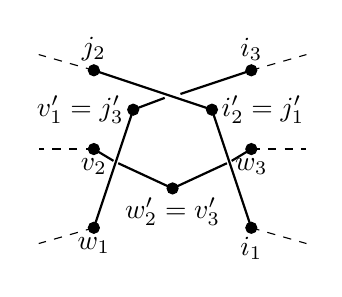
\begin{tikzpicture}
\draw[dashed] (-1,-1) -- (-1.7,-1.2);
\draw[dashed] (-1,0) -- (-1.7,0);
\draw[dashed] (-1,1) -- (-1.7,1.2);
\draw[dashed] (1,0) -- (1.7,0);
\draw[dashed] (1,1) -- (1.7,1.2);
\draw[dashed] (1,-1) -- (1.7,-1.2);
\draw[black, thick] (-1,-1) -- (-0.5,0.5);
\draw[black, thick] (-1,0) -- (-0.75,-0.15);
\draw[black, thick] (-0.69,-0.18) -- (0,-0.5);
\draw[black, thick] (-1,1) -- (0.5,0.5);
\draw[black, thick] (1,0) -- (0.75,-0.15);
\draw[black, thick] (0.69,-0.18) -- (0,-0.5);
\draw[black, thick] (1,1) -- (0.1,0.7);
\draw[black, thick] (-0.1,0.65) -- (-0.5,0.5);
\draw[black, thick] (1,-1) -- (0.5,0.5);
\filldraw[black] (-1,1) circle (2pt) node[anchor=south]{$j_2$};
\filldraw[black] (0,-0.5) circle (2pt) node[anchor=north]{$w_{2}'=v_{3}'$};
\filldraw[black] (1,1) circle (2pt) node[anchor=south]{$i_3$};
\filldraw[black] (-1,0) circle (2pt) node[anchor=north]{$v_2$};
\filldraw[black] (1,0) circle (2pt) node[anchor=north]{$w_3$};
\filldraw[black] (0.5,0.5) circle (2pt) node[anchor=west]{$i_{2}'=j_{1}'$};
\filldraw[black] (-0.5,0.5) circle (2pt) node[anchor=east]{$v_{1}'=j_{3}'$};
\filldraw[black] (-1,-1) circle (2pt) node[anchor=north]{$w_1$};
\filldraw[black] (1,-1) circle (2pt) node[anchor=north]{$i_1$};
\end{tikzpicture}};\\
};
\end{tikzpicture}
\caption{The polygonal Reidemeister III move: the initial diagram (left) and the deformed diagram (right).}
\label{fig14}
\end{figure}
 

\section*{Acknowledgements}

The author was supported by the Slovenian Research Agency grants P1-0292, N1-0278 and J1-4031.



\begin{thebibliography}{1}

%\bibitem{CAL} J. A. Calvo, {\em Geometric knot spaces and polygonal isotopy}, Journal of knot theory and its ramifications, 10 (02), 245--267, 2001. 

\bibitem{BN} D. Bar-Natan, {\em Khovanov's homology for tangles and cobordisms}, Geometry \& Topology, 9, 1443--1499, 2005.

\bibitem{LIV} C. Livingston, {\em Knot theory}, The Mathematical Association of America, 1993. 

\bibitem{TUR} P. Turner, {\em Five lectures on Khovanov homology}, arXiv:math/0606464v1[math-GT], 2006.

\end{thebibliography}




\end{document}

